\newpage
\section{Projekt sieci}
\paragraph{}
Kolejnym etapem naszego projektu jest projekt logiczny sieci. Na Rysunku \textbf{TODO} przedstawiony zostało wzajemne położenie względem siebie budynków, które dla ulatwienia oznaczeń nazywać i opisu nazywać będziemy \textit{B1} i \textit{B2}.

\subsection{Projekt logiczny sieci}
\paragraph{}
Ze względu na charakterystykę działania firmy i potrzeby odbiorcy, sieć podzielona została na sieci \textit{VLany}, odpowiadające każdemu zespołowi programistów. Pozwoli to na łatwe dołączanie osób do różnych zespołów (np. testerów oprogramowania), bez konieczności fizycznego przenoszenia komputea do pomieszczenia danego zespołu.

\paragraph{}
Na każdym piętrze dostepna będzie drukarka sieciowa, posiadająca adres z puli odpowedniego \textit{VLanu}.

\paragraph{}
W celu zapewnienia płynnego ruchu sieciowego na każdym piętrze znajdować sie będzie switch warstwy 2, podpiety do dwóch przełączników warstwy trzeciej znajdujących się an parterze każdego z budynków. Pomiędzy przełącznikami warstwy trzeciej skonfigurowane zostanie funkcja EtherChannel, pozwalający na połączeniu kilku ethernetowych łączy fizycznych w jedno logiczne. Dzięki temu, przełączniki mogą równomiernie rozkładać obciążenie na łączu, zapewnieniają wysokowydajnościowe połączenie pomiędzy urządzeniami sieciowymi.

\paragraph{}
Przełączniki warstwy trzeciej połączone ze sobą zostaną światłowodem w połączeniu każdy z każdym, by zapewnić niezawodność połączenia i zminimalizować ryzyko braku połączenia do internetu lub serwerowni \textit{B2} w wyniku awarii switch'a.

\paragraph{}
Dwa routery znjadujące się w \textit{B1} odpowiedzialne będą za zapewnienie niezawodnego połączenia z internetem. Pomiędzy ruoterami zastosowany zosatnie protokół VRRP, pozwalający na stworzenie klastra dostępowego, określanego jako wirtualny router. Przyśieszy to ruch sieciowy, oraz zwiększy bezpieczeństwo i niezawodność połączenia z internetem.

\newpage
\paragraph{}
Oznaczenia :
\begin{itemize}
	\item B\{X\}S\{Y\} - Switch warstwy 2, gdzie \{X\} - numer budynku, \{Y\} - numer piętra
	\item B\{X\}RS\{Y\} - Switch warstwy 3, gdzie \{X\} - numer budynku, \{Y\} - numer urządzenia
	\item R\{X\} - Router, gdzie \{X\} - numer urządzenia
	\item S\{X\} - Serwer, gdzie \{X\} - numer urządzenia
	\item B\{X\}P\{Y\}A\{Z\} - Access Point, gdzie \{X\} - numer budynku, \{Y\} - numer piętra, \{Z\} - numer urządzenie
	\item B\{X\}P\{Y\}K\{Z\} - Stacja robocza, gdzie \{X\} - numer budynku, \{Y\} - numer piętra, \{Z\} - numer urządzenie
	\item B\{X\}P\{Y\}D\{Z\} - Drukarka sieciowa, gdzie \{X\} - numer budynku, \{Y\} - numer piętra, \{Z\} - numer urządzenie
	\item FW\{X\} - Firewall sprzętowy, gdzie \{X\} - numer urządzenia
\end{itemize}

\newpage
\begin{figure}[H]
  \begin{center}
    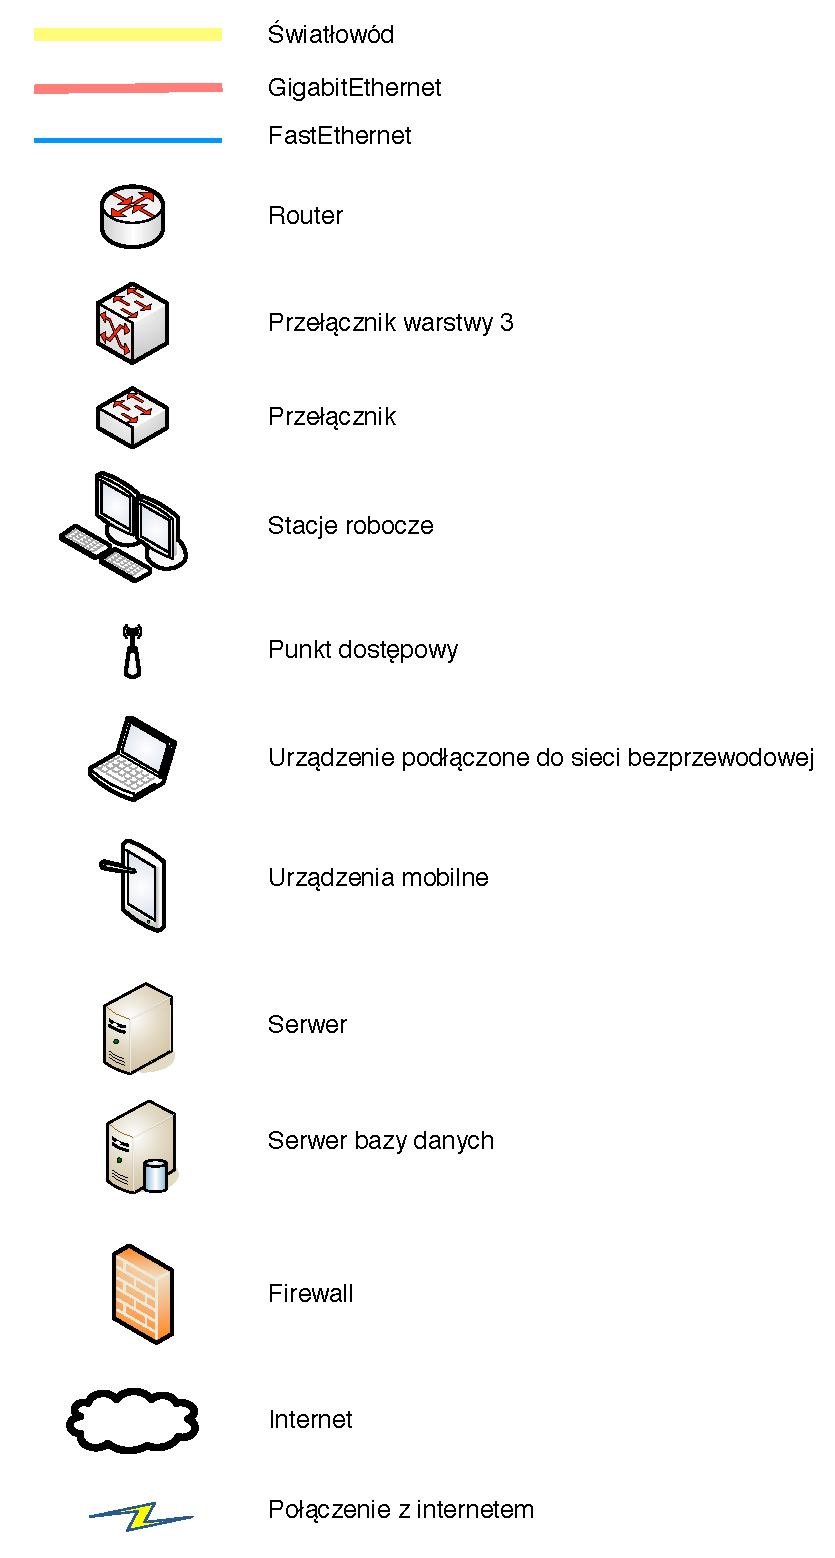
\includegraphics[scale = 0.7]{img/schemat-legenda.pdf}
    \caption{Schemat logiczny - legenda}
  \end{center}
\end{figure}

\newpage
\begin{figure}[H]
  \begin{center}
    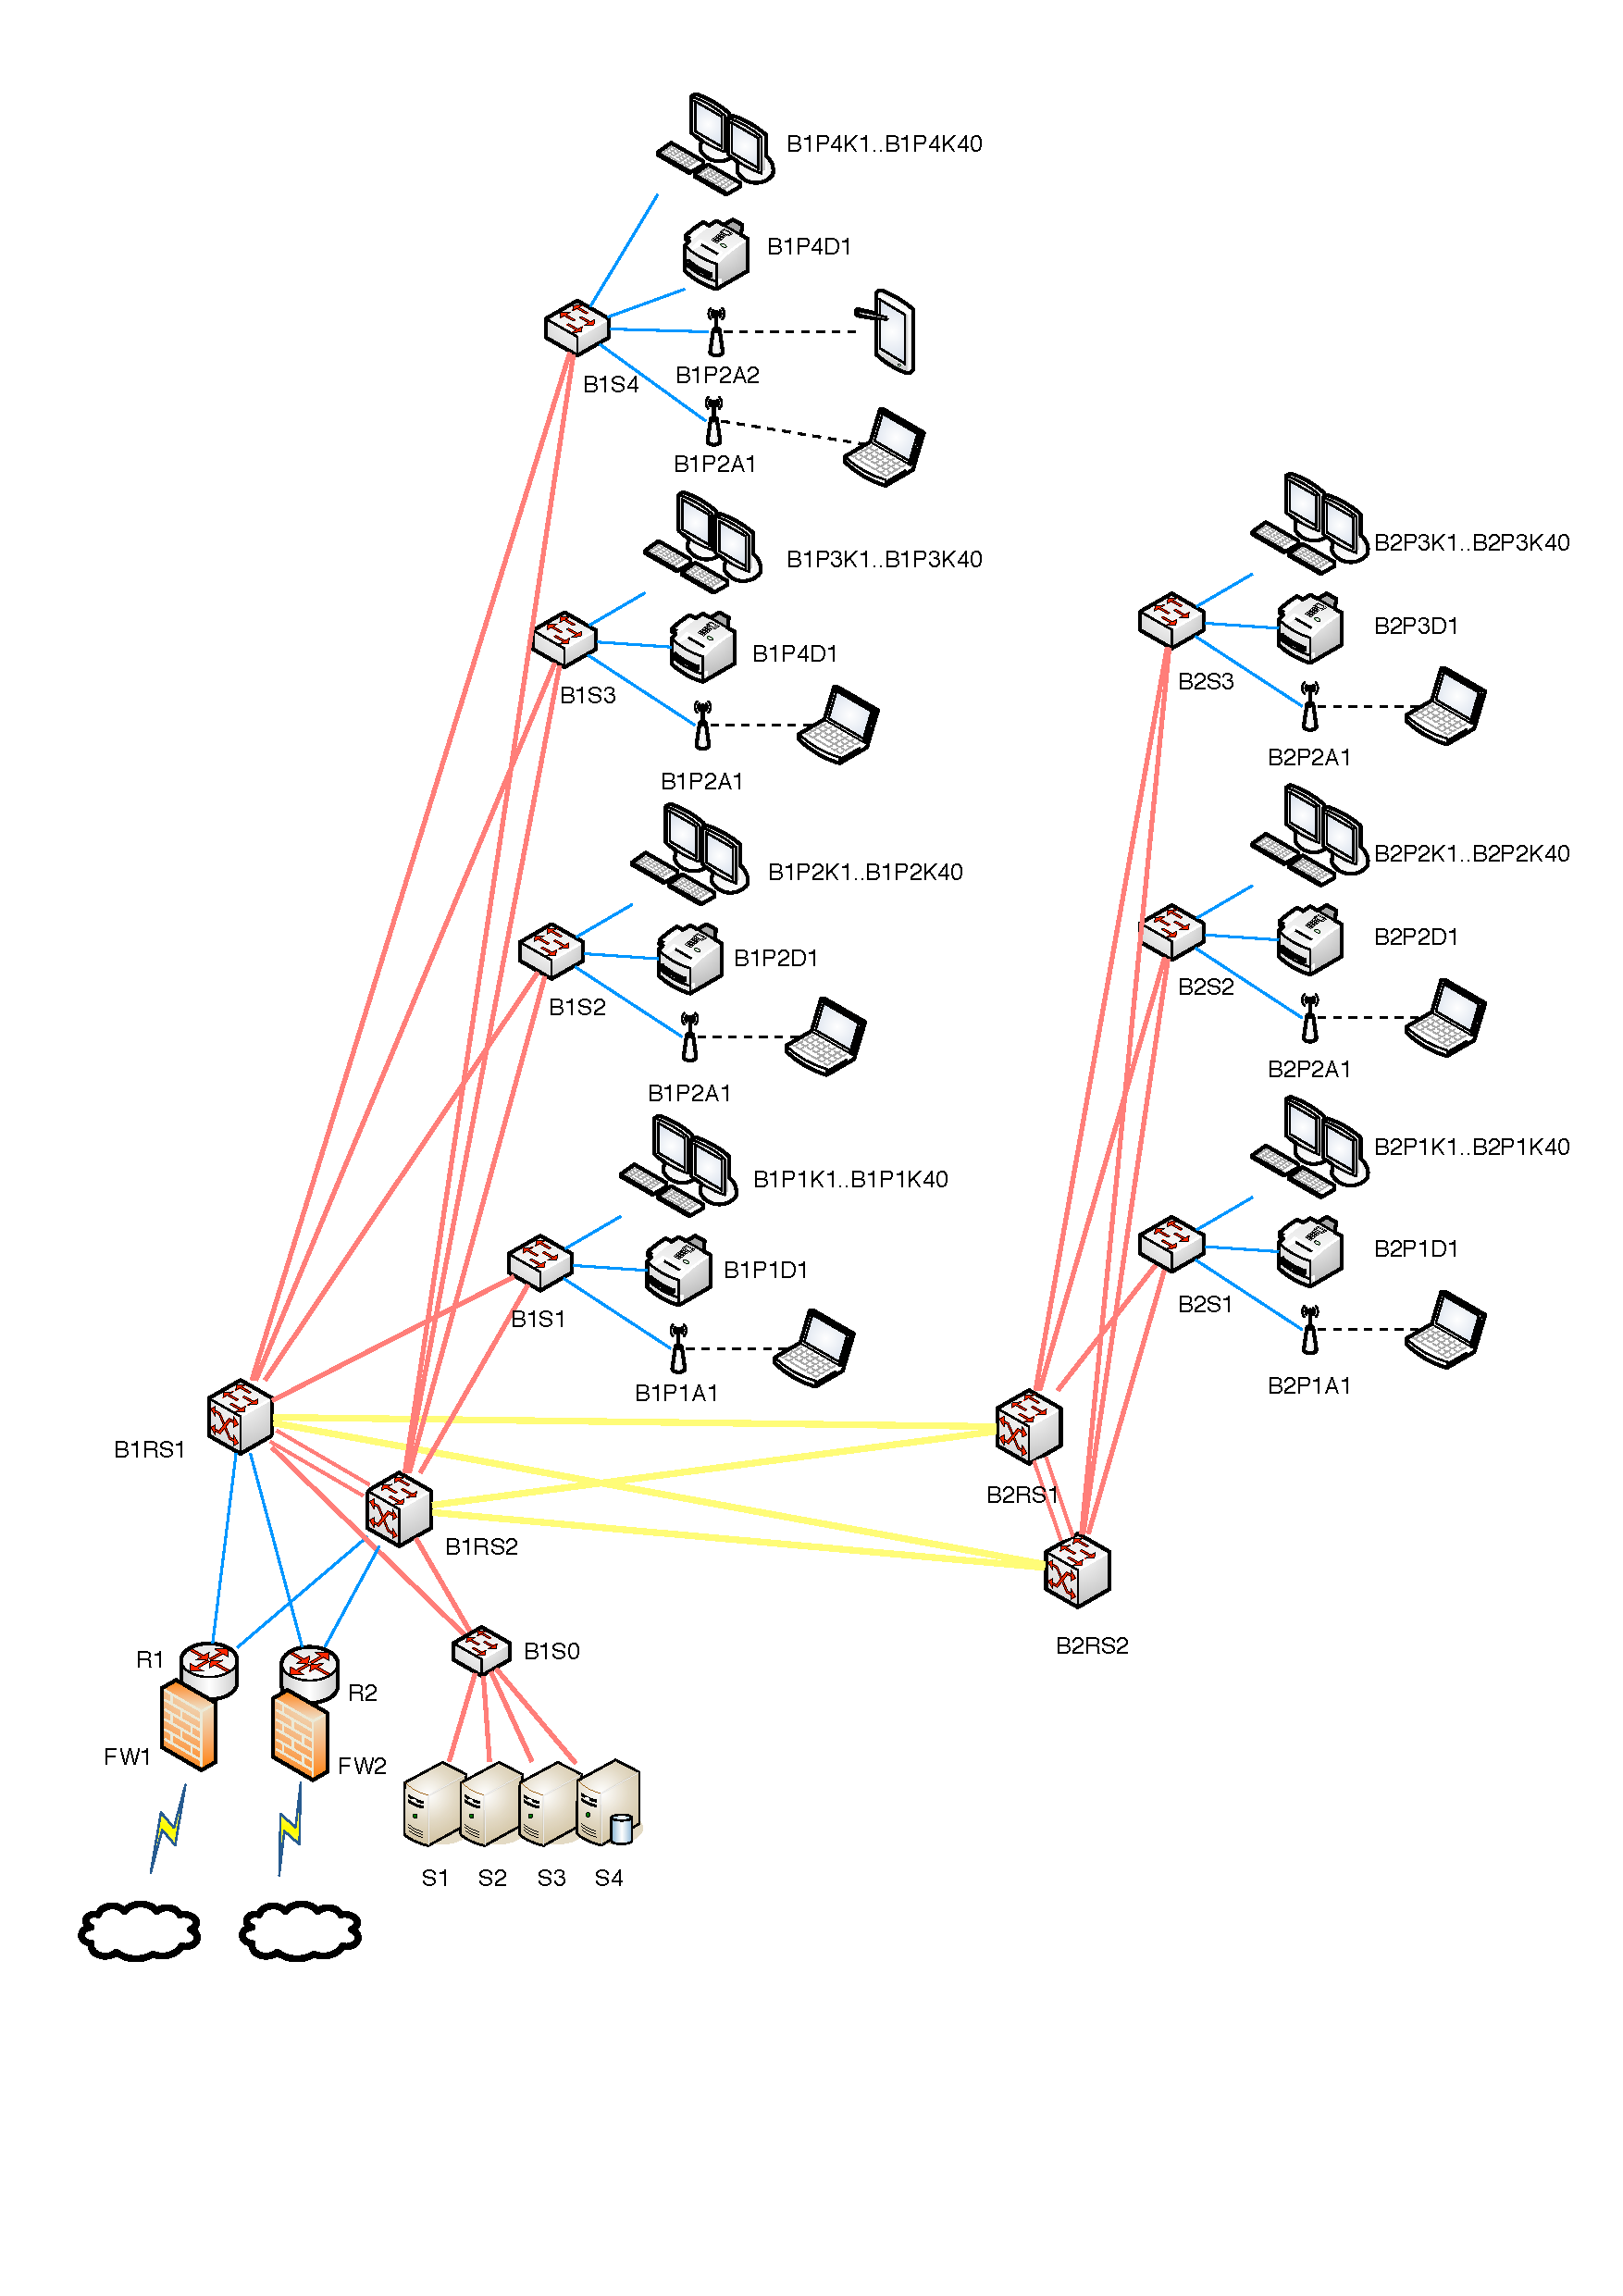
\includegraphics[width=\textwidth]{img/schemat.pdf}
    \caption{Schemat logiczny}
  \end{center}
\end{figure}


\paragraph{}
Podział na Vlany :
\begin{itemize}
	\item VLan WiFi - grupujący użytkowników zewnętrznych (np. klientów), niemających dostępu do zasobów wewnętrznych sieci
	\item VLan ZarzadIAdministracja - grupujący pracowników z działu Administracyjnego, HR oraz zarząd firmy
	\item VLan Team\{X\} - (\{X\} numer zespołu) grupujący członków danego zespołu
	\item VLan UrzadzeniaMobilne - grupujący urządzenia mobilne, wykorzystywane przez programistów aplikacji na przenośne aparaty
	\item VLan Serwerownia - grupujący serwery
\end{itemize}

\subsection{Konfiguracja adresacji \textit{IP}}
\paragraph{}
W celu zapewnienia odpowiedniej puli adresów, zapewniajacej możliwość skalowalności i robudowy sieci (np o nowe switche na poszczególnych pietrach) zdecydowaliśmy się na pulę adresów prywatnych klasy A, zaczynając od adresu sieci \textit{10.1.1.0}.
\paragraph{}
Poniżej przedstawiono pule adresowe dla poszczególnych \textit{VLanów} :
\begin{itemize}
	\item VLan WiFi : 10.1.1.0 - 10.1.1.255, Adres sieci : 10.1.1.0, Broadcast : 10.1.1.255, Maska : 255.255.255.0
	\item VLan ZarzadIAdministracja : 10.1.2.0 - 10.1.2.255, Adres sieci : 10.1.2.0, Broadcast : 10.1.2.255, Maska : 255.255.255.0
	\item VLan Team1 10.1.3.0 - 10.1.3.255, Adres sieci : 10.1.3.0, Broadcast : 10.1.3.255, Maska : 255.255.255.0
	\item VLan Team2 10.1.4.0 - 10.1.4.255, Adres sieci : 10.1.4.0, Broadcast : 10.1.4.255, Maska : 255.255.255.0
	\item VLan Team3 10.1.5.0 - 10.1.5.255, Adres sieci : 10.1.5.0, Broadcast : 10.1.5.255, Maska : 255.255.255.0
	\item VLan Team4 10.1.6.0 - 10.1.6.255, Adres sieci : 10.1.6.0, Broadcast : 10.1.6.255, Maska : 255.255.255.0
	\item VLan Team5(Testerzy) 10.1.7.0 - 10.1.7.255, Adres sieci : 10.1.7.0, Broadcast : 10.1.7.255, Maska : 255.255.255.0
	\item VLan UrzadzeniaMobilne 10.1.8.0 - 10.1.8.255, Adres sieci : 10.1.8.0, Broadcast : 10.1.8.255, Maska : 255.255.255.0
	\item VLan Serwerownia 10.1.9.0 - 10.1.9.255, Adres sieci : 10.1.9.0, Broadcast : 10.1.9.255, Maska : 255.255.255.0
\end{itemize}


\subsection{Projekt fizyczny}
\paragraph{}
Na każdym piętrze obu budynków, poza parterem, znajdować się będą naścienne szafy 4U, w których umieszczone zosatną przełączniki warstwy drugiej oraz po dwa patch panele każdy posiadający 24 porty.
\paragraph{}

\subsubsection{Projekt okablowania}
\begin{figure}[H]
  \begin{center}
    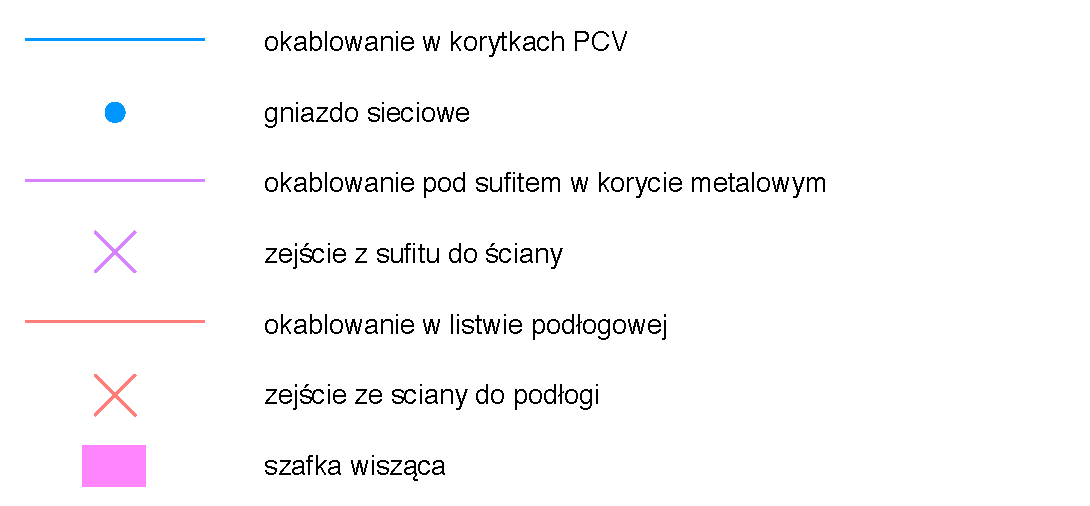
\includegraphics[width=\textwidth]{img/s/legenda.pdf}
    \caption{Schemat okablowania - legenda}
  \end{center}
\end{figure}


\newpage
\begin{figure}[H]
  \begin{center}
    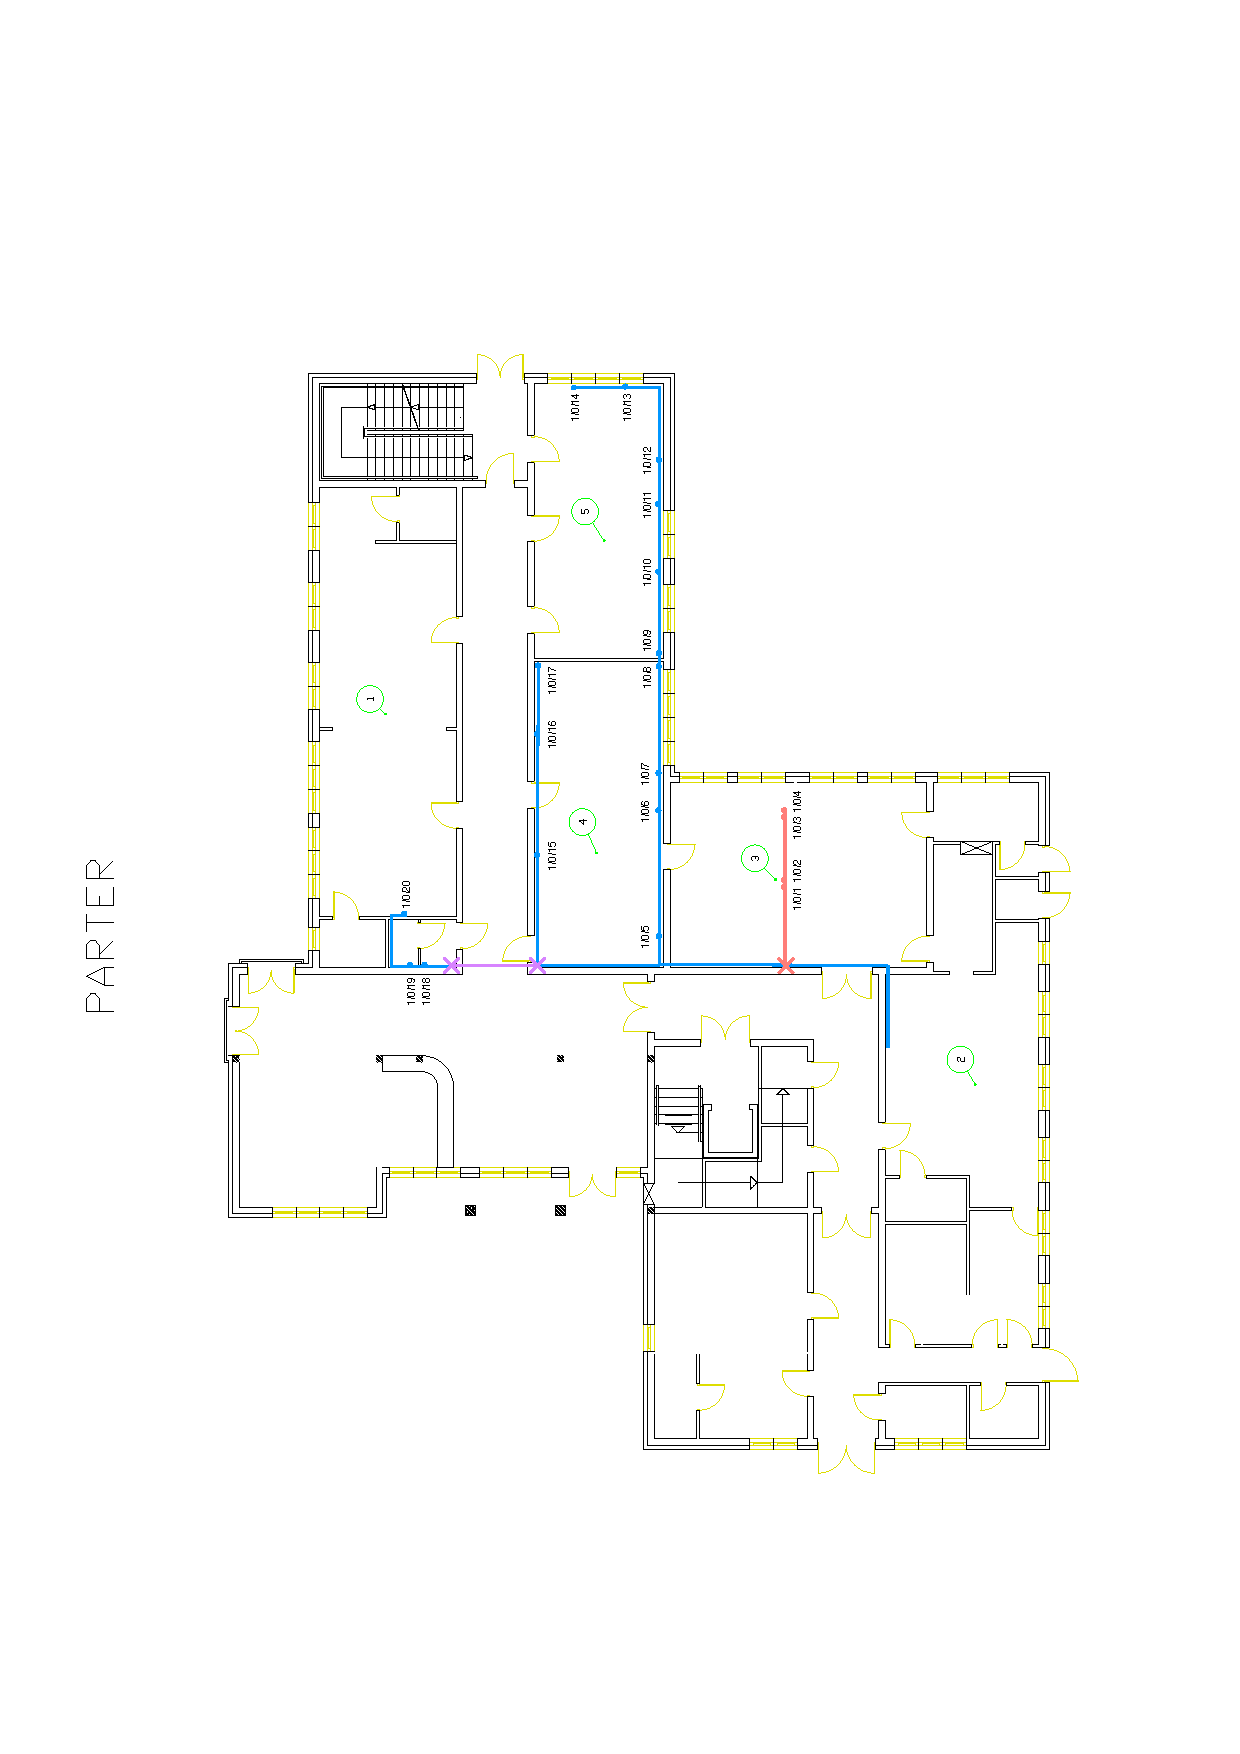
\includegraphics[width=\textwidth]{img/s/b1-0.pdf}
    \caption{Budynek 1 - Parter}
  \end{center}
\end{figure}

\begin{figure}[H]
  \begin{center}
    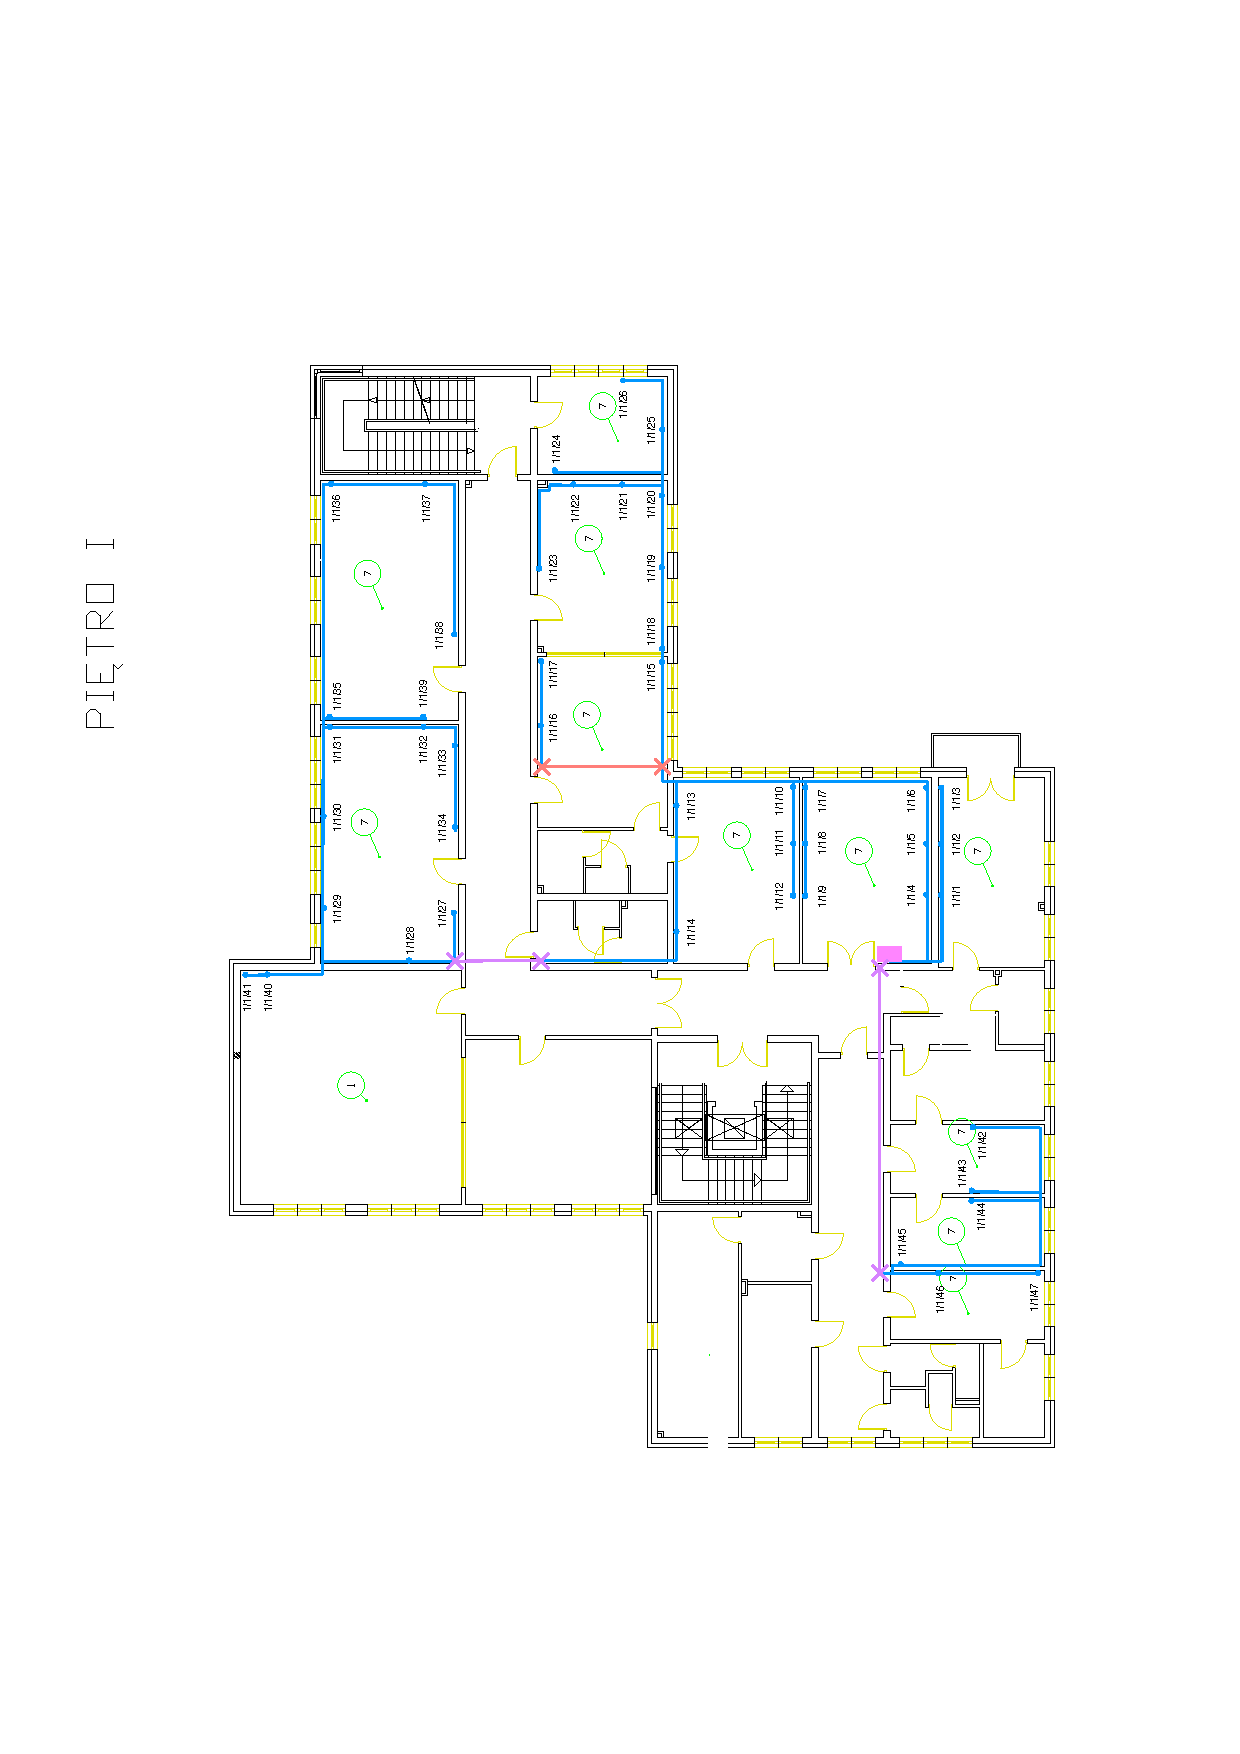
\includegraphics[width=\textwidth]{img/s/b1-1.pdf}
    \caption{Budynek 1 - Piętro I}
  \end{center}
\end{figure}

\begin{figure}[H]
  \begin{center}
    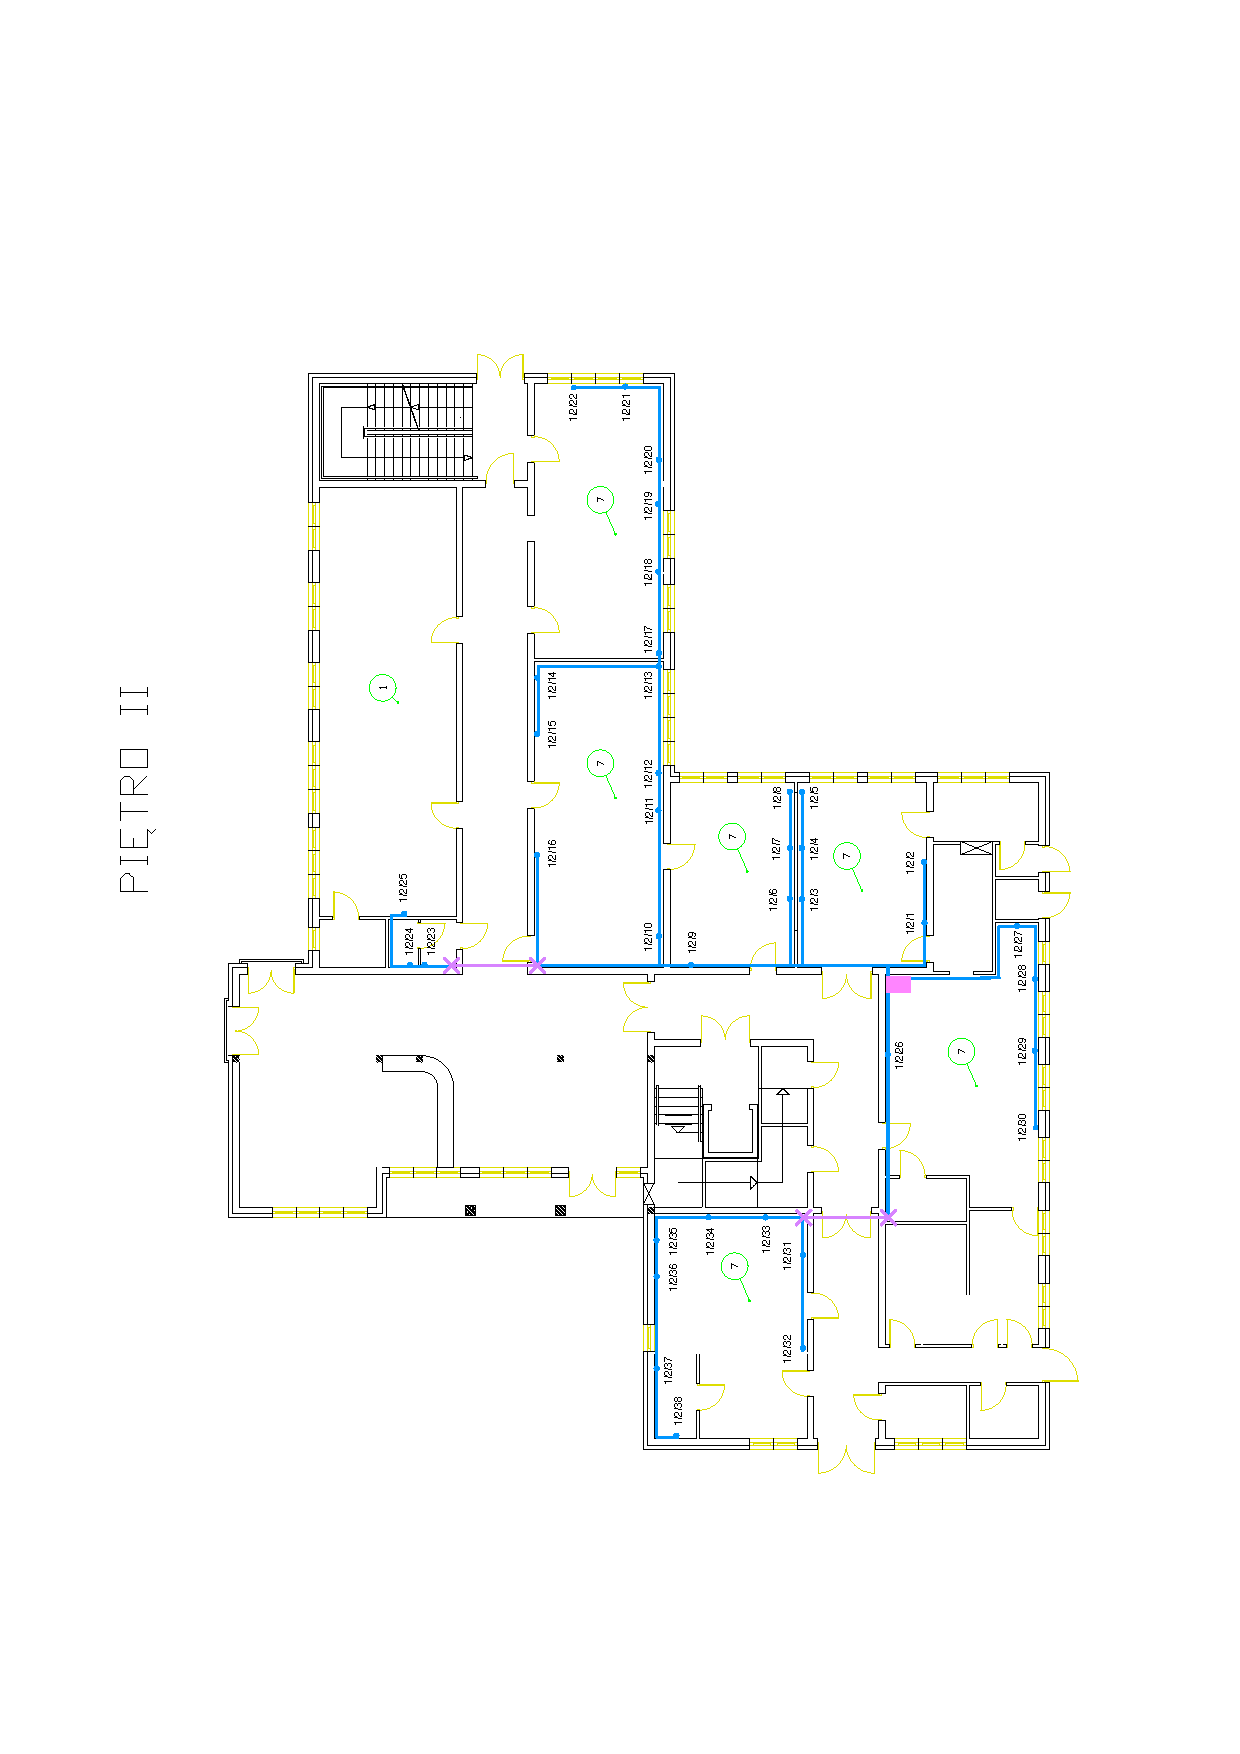
\includegraphics[width=\textwidth]{img/s/b1-2.pdf}
    \caption{Budynek 1 - Piętro II}
  \end{center}
\end{figure}

\begin{figure}[H]
  \begin{center}
    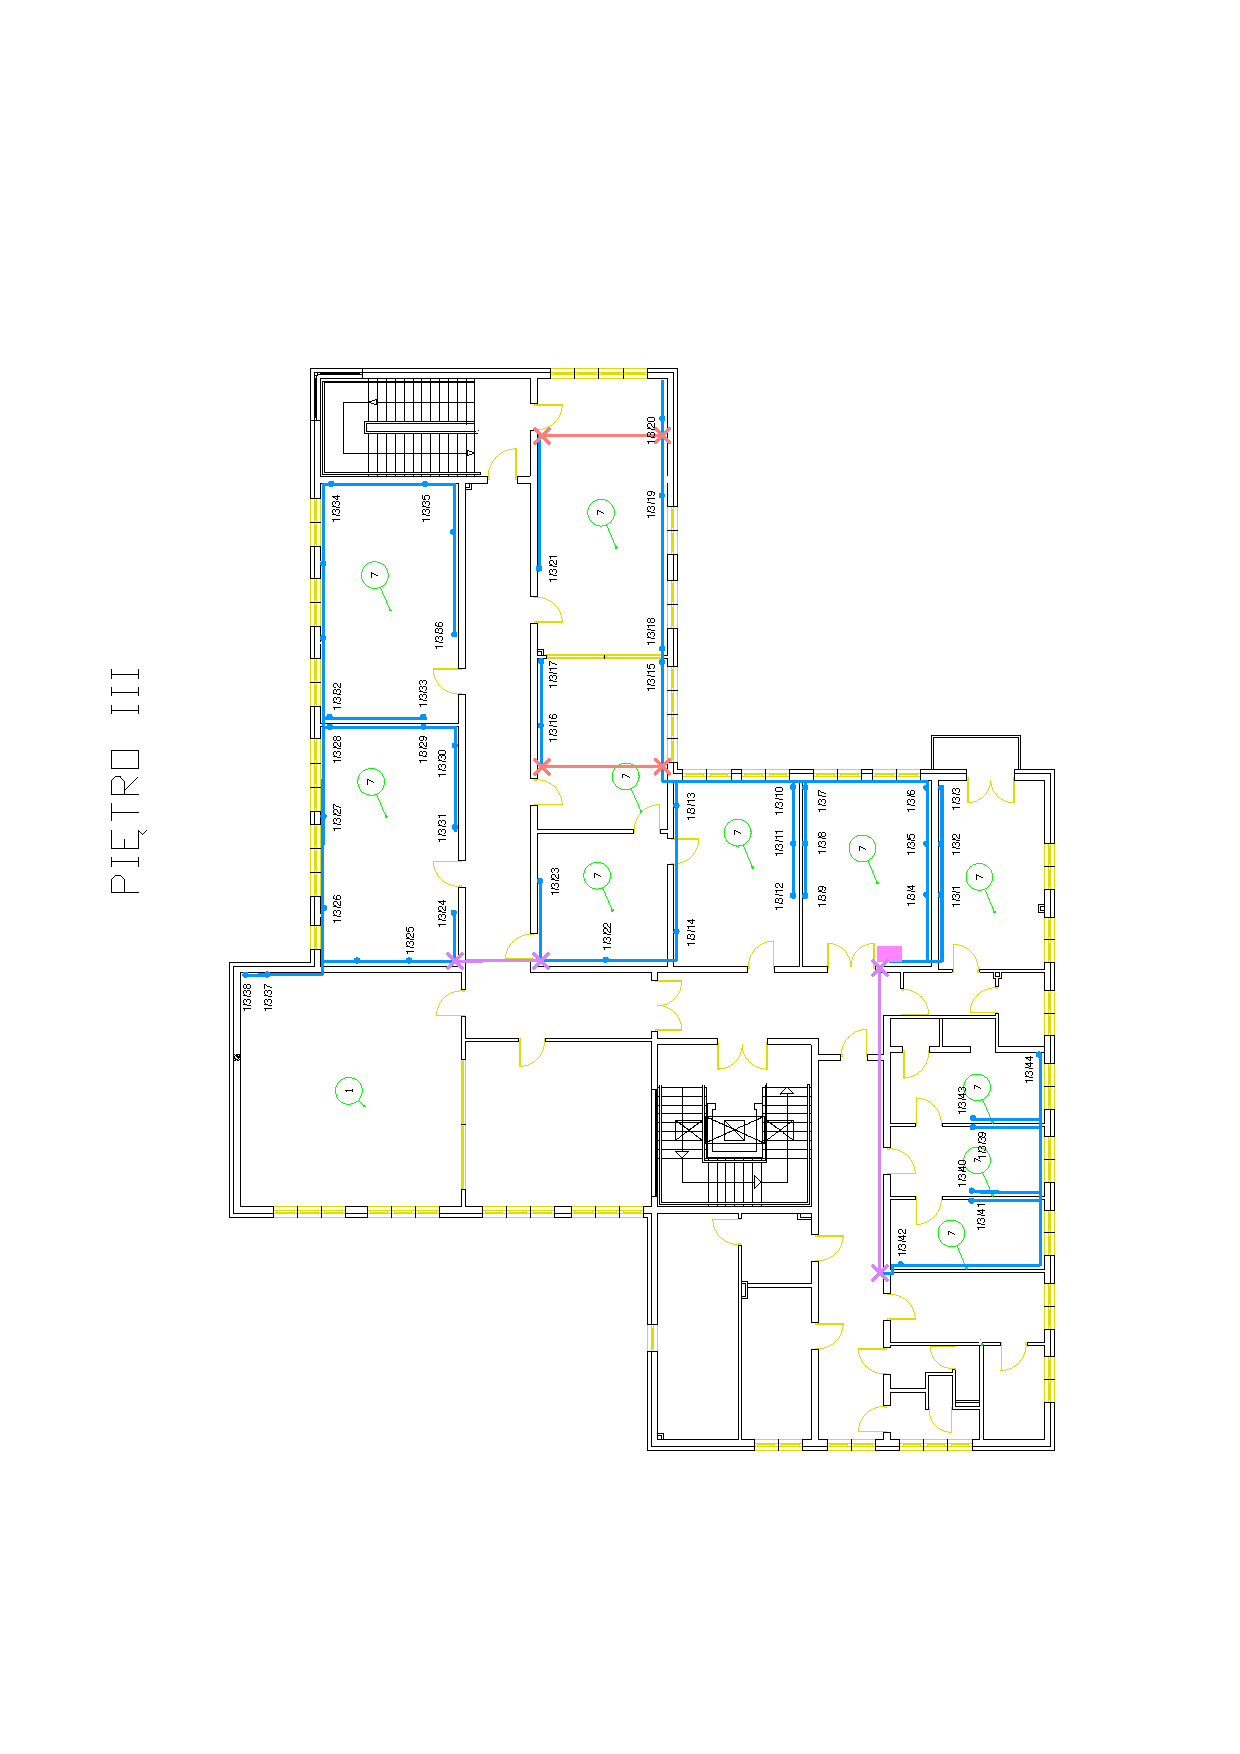
\includegraphics[width=\textwidth]{img/s/b1-3.pdf}
    \caption{Budynek 1 - Piętro III}
  \end{center}
\end{figure}

\begin{figure}[H]
  \begin{center}
    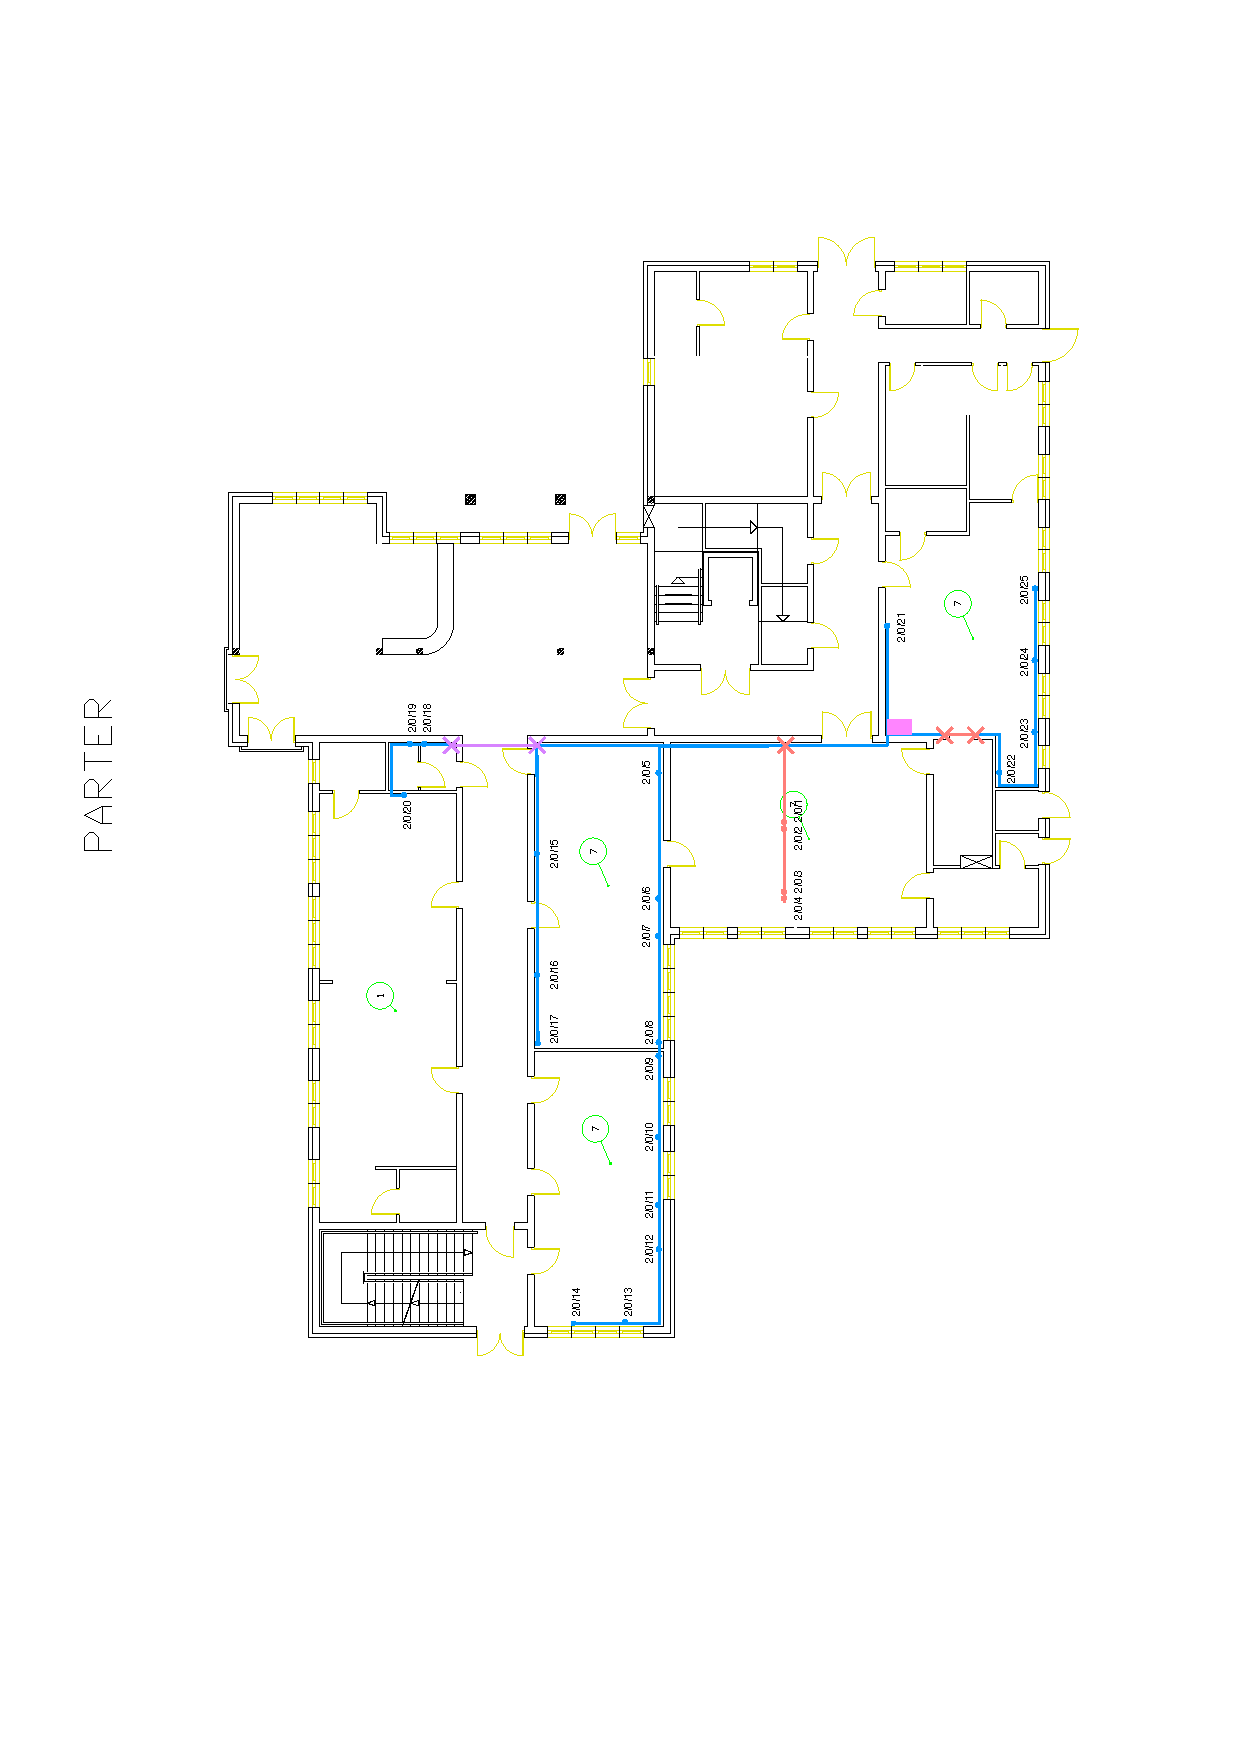
\includegraphics[width=\textwidth]{img/s/b2-0.pdf}
    \caption{Budynek 2 - Parter}
  \end{center}
\end{figure}

\begin{figure}[H]
  \begin{center}
    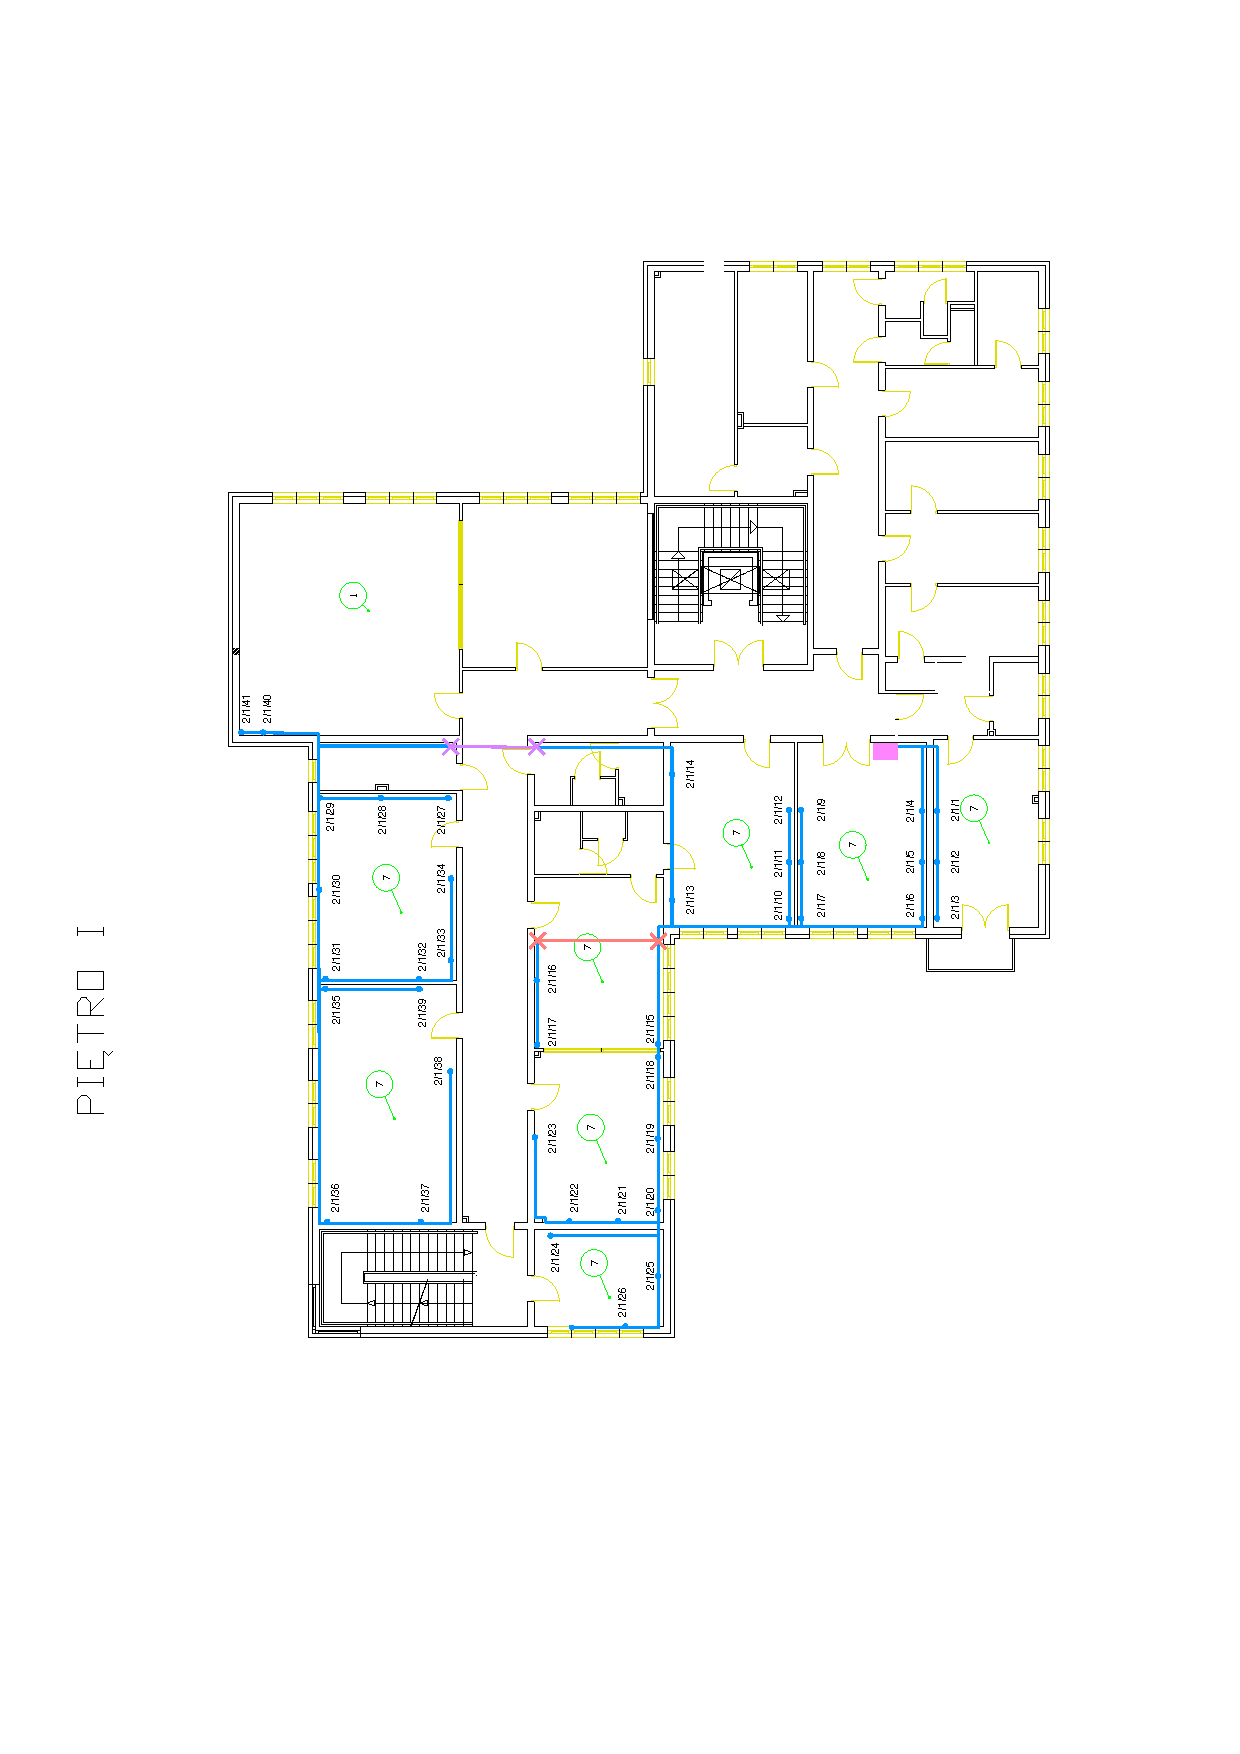
\includegraphics[width=\textwidth]{img/s/b2-1.pdf}
    \caption{Budynek 2 - Piętro I}
  \end{center}
\end{figure}

\begin{figure}[H]
  \begin{center}
    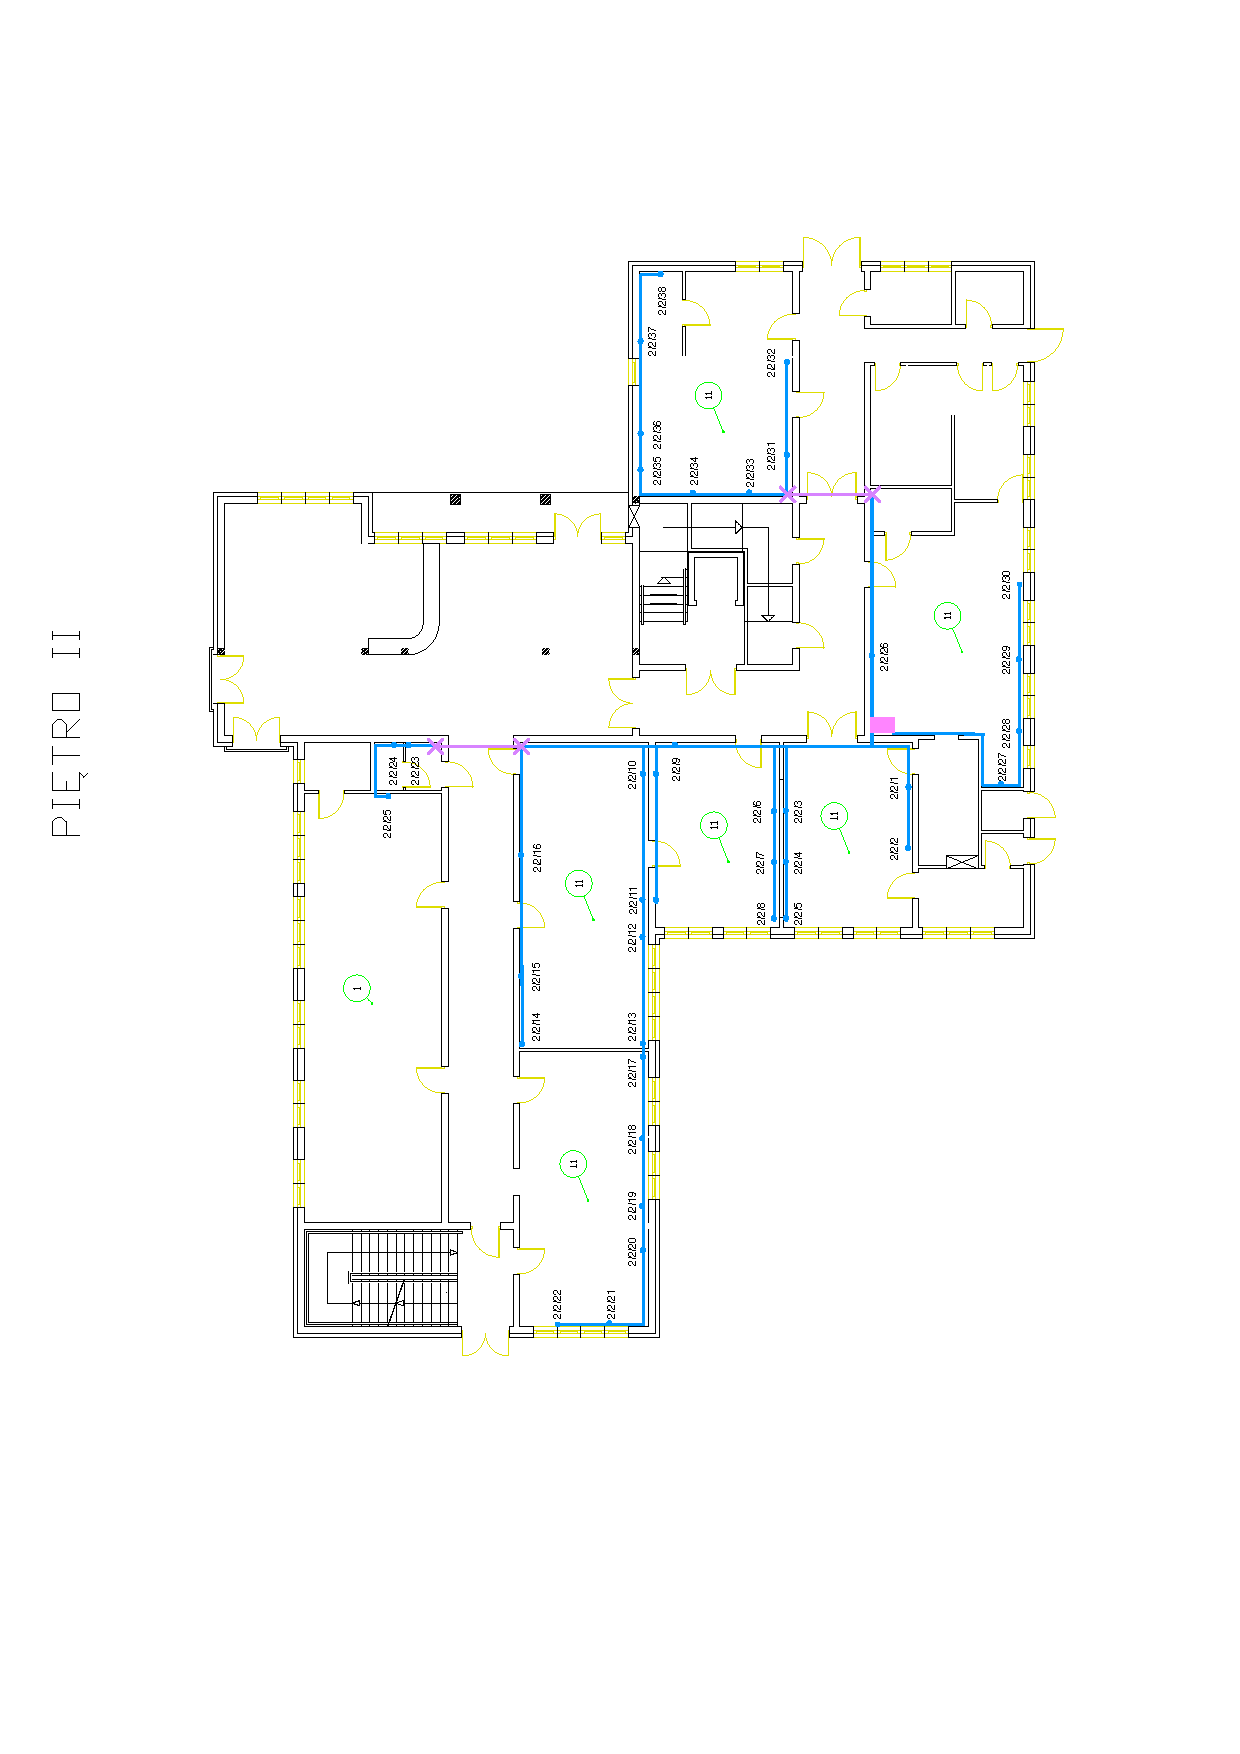
\includegraphics[width=\textwidth]{img/s/b2-2.pdf}
    \caption{Budynek 2 - Piętro II}
  \end{center}
\end{figure}


\subsubsection{Umiejscownienie urządzeń w szafach}


\paragraph{}
Na piętrach 1-3 budynku B1 oraz 1,2 budynku B2 umieszczone zostały identyczne szafy wiszące (4U), każda z nich zawiera przełącznik warstwy drugiej oraz dwa 24-portowe patch panele.

\begin{figure}[H]
  \begin{center}
    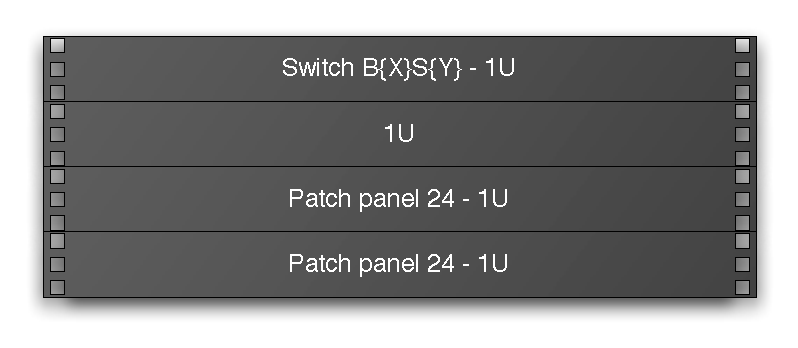
\includegraphics[width=\textwidth]{img/s/szafa-mala.pdf}
    \caption{Schemat szafy wiszącej}
  \end{center}
\end{figure}

\paragraph{}
W serwerowni mieszczącej się na parterze budynku B1 została umieszczona szafa stojąca (15U).
Zawiera ona przełączniki: B1S0 - podłączony do serwerów oraz B1S1 wraz z dwoma 24-portowymi patch panelami, który łączy z siecią komputery z parteru.
Ponadto w szafie znajdują się przełączniki warsty trzeciej, routery wraz z firewallami, serwery, a także awaryjny zasilcz..


\begin{figure}[H]
  \begin{center}
    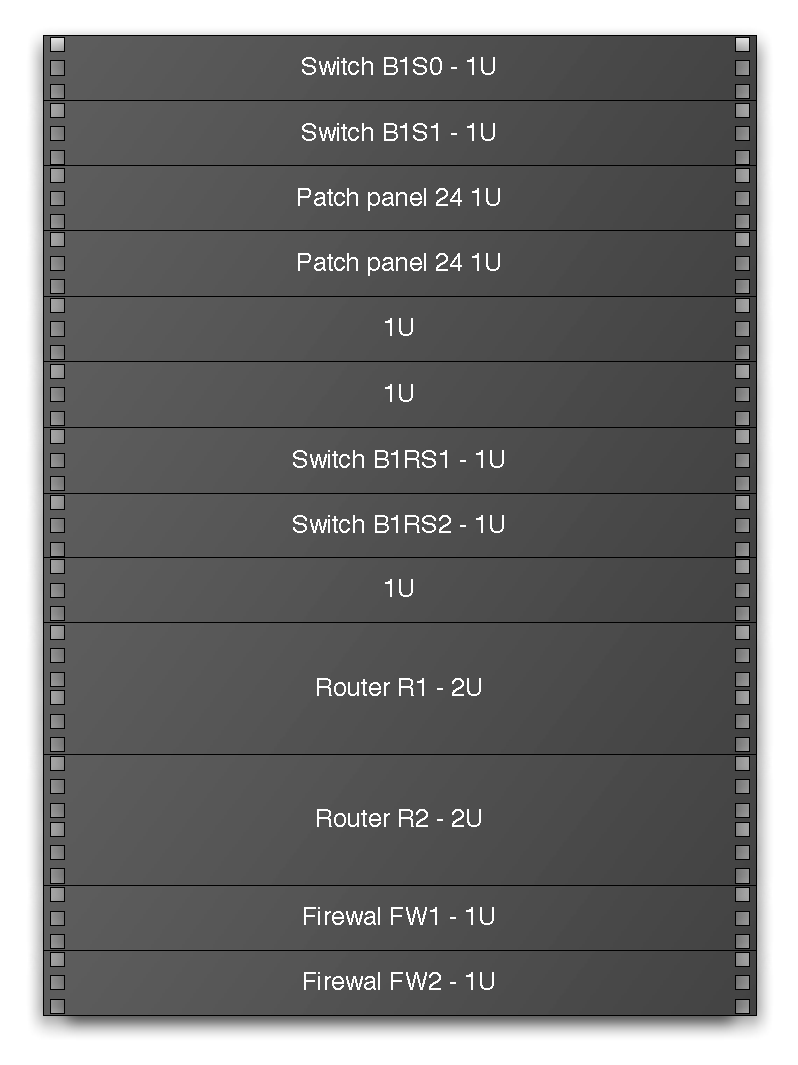
\includegraphics[width=\textwidth]{img/s/szafa-b1.pdf}
    \caption{Schemat szafy stojącej na parterze budynku B1}
  \end{center}
\end{figure}

\paragraph{}
Na parterze budynku B2 znajduje się większa szafa niż na piętrach, wynika to z konieczności umieszczenia przełączników warstwy trzeciej.

\begin{figure}[H]
  \begin{center}
    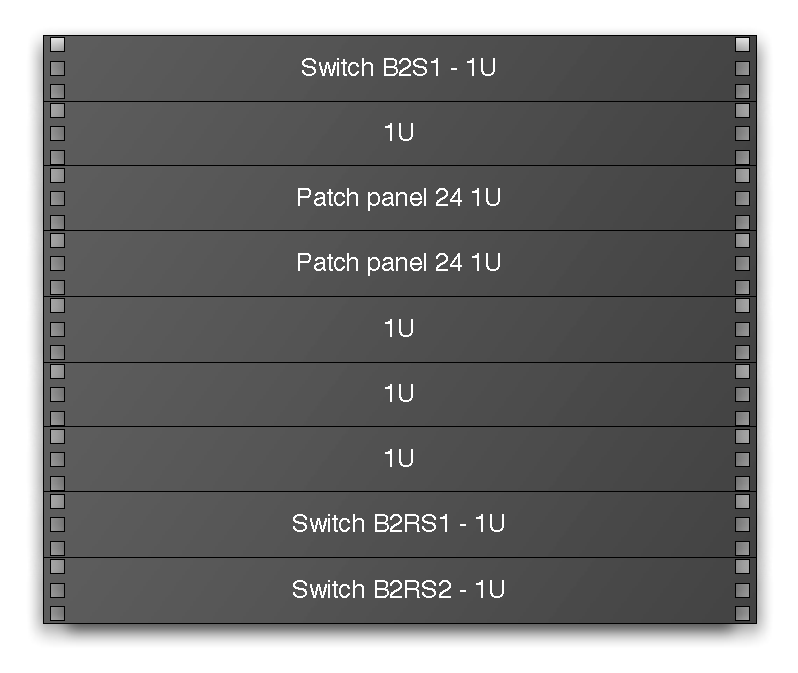
\includegraphics[width=\textwidth]{img/s/szafa-b2.pdf}
    \caption{Schemat szafy wiszącej na parterze budynku B2}
  \end{center}
\end{figure}


\subsubsection{Tabela połączeń}
\paragraph{}
Poniższe tabele prezentują sposób w jaki zostały przyporządkowane gniazda do kolejnych portów przełącznika warstwy drugiej dla poszczególnych pięter w budynkach.
\begin{center}
    \begin{longtable}{|c|c|c|c|c|}
    \hline
    Gniazdo & Port Switch & Switch & Odległość \\ \hline
	1/0/1 & Fa0/1 & B1S1 & dupa \\ \hline
	1/0/2 & Fa0/2 & B1S1 & dupa \\ \hline
	1/0/3 & Fa0/3 & B1S1 & dupa \\ \hline
	1/0/4 & Fa0/4 & B1S1 & dupa \\ \hline
	1/0/5 & Fa0/5 & B1S1 & dupa \\ \hline
	1/0/6 & Fa0/6 & B1S1 & dupa \\ \hline
	1/0/7 & Fa0/7 & B1S1 & dupa \\ \hline
	1/0/8 & Fa0/8 & B1S1 & dupa \\ \hline
	1/0/9 & Fa0/9 & B1S1 & dupa \\ \hline
	1/0/10 & Fa0/10 & B1S1 & dupa \\ \hline
	1/0/11 & Fa0/11 & B1S1 & dupa \\ \hline
	1/0/12 & Fa0/12 & B1S1 & dupa \\ \hline
	1/0/13 & Fa0/13 & B1S1 & dupa \\ \hline
	1/0/14 & Fa0/14 & B1S1 & dupa \\ \hline
	1/0/15 & Fa0/15 & B1S1 & dupa \\ \hline
	1/0/16 & Fa0/16 & B1S1 & dupa \\ \hline
	1/0/17 & Fa0/17 & B1S1 & dupa \\ \hline
	1/0/18 & Fa0/18 & B1S1 & dupa \\ \hline
	1/0/19 & Fa0/19 & B1S1 & dupa \\ \hline
	1/0/20 & Fa0/20 & B1S1 & dupa \\ \hline
	1/0/21 & Fa0/21 & B1S1 & dupa \\ \hline
	1/0/22 & Fa0/22 & B1S1 & dupa \\ \hline
	1/0/23 & Fa0/23 & B1S1 & dupa \\ \hline
	1/0/24 & Fa0/24 & B1S1 & dupa \\ \hline
	1/0/25 & Fa0/25 & B1S1 & dupa \\ \hline
	1/0/26 & Fa0/26 & B1S1 & dupa \\ \hline
	1/0/27 & Fa0/27 & B1S1 & dupa \\ \hline
	1/0/28 & Fa0/28 & B1S1 & dupa \\ \hline
	1/0/29 & Fa0/29 & B1S1 & dupa \\ \hline
	1/0/30 & Fa0/30 & B1S1 & dupa \\ \hline
	1/0/31 & Fa0/31 & B1S1 & dupa \\ \hline
	1/0/32 & Fa0/32 & B1S1 & dupa \\ \hline
	1/0/33 & Fa0/33 & B1S1 & dupa \\ \hline
	1/0/34 & Fa0/34 & B1S1 & dupa \\ \hline
	1/0/35 & Fa0/35 & B1S1 & dupa \\ \hline
	1/0/36 & Fa0/36 & B1S1 & dupa \\ \hline
	1/0/37 & Fa0/37 & B1S1 & dupa \\ \hline
	1/0/38 & Fa0/38 & B1S1 & dupa \\ \hline
	1/0/39 & Fa0/39 & B1S1 & dupa \\ \hline
	1/0/40 & Fa0/40 & B1S1 & dupa \\ \hline
	1/0/41 & Fa0/41 & B1S1 & dupa \\ \hline
	1/0/42 & Fa0/42 & B1S1 & dupa \\ \hline
	1/0/43 & Fa0/43 & B1S1 & dupa \\ \hline
	1/0/44 & Fa0/44 & B1S1 & dupa \\ \hline
	1/0/45 & Fa0/45 & B1S1 & dupa \\ \hline
	1/0/46 & Fa0/46 & B1S1 & dupa \\ \hline
	1/0/47 & Fa0/47 & B1S1 & dupa \\ \hline
	1/0/48 & Fa0/48 & B1S1 & dupa \\ \hline

    \end{longtable}
\end{center}

\begin{center}
    \begin{longtable}{|c|c|c|c|c|}
    \hline
    Gniazdo & Port Switch & Switch & Odległość \\ \hline
	1/1/1 & Fa0/1 & B1S2 & dupa \\ \hline
	1/1/2 & Fa0/2 & B1S2 & dupa \\ \hline
	1/1/3 & Fa0/3 & B1S2 & dupa \\ \hline
	1/1/4 & Fa0/4 & B1S2 & dupa \\ \hline
	1/1/5 & Fa0/5 & B1S2 & dupa \\ \hline
	1/1/6 & Fa0/6 & B1S2 & dupa \\ \hline
	1/1/7 & Fa0/7 & B1S2 & dupa \\ \hline
	1/1/8 & Fa0/8 & B1S2 & dupa \\ \hline
	1/1/9 & Fa0/9 & B1S2 & dupa \\ \hline
	1/1/10 & Fa0/10 & B1S2 & dupa \\ \hline
	1/1/11 & Fa0/11 & B1S2 & dupa \\ \hline
	1/1/12 & Fa0/12 & B1S2 & dupa \\ \hline
	1/1/13 & Fa0/13 & B1S2 & dupa \\ \hline
	1/1/14 & Fa0/14 & B1S2 & dupa \\ \hline
	1/1/15 & Fa0/15 & B1S2 & dupa \\ \hline
	1/1/16 & Fa0/16 & B1S2 & dupa \\ \hline
	1/1/17 & Fa0/17 & B1S2 & dupa \\ \hline
	1/1/18 & Fa0/18 & B1S2 & dupa \\ \hline
	1/1/19 & Fa0/19 & B1S2 & dupa \\ \hline
	1/1/20 & Fa0/20 & B1S2 & dupa \\ \hline
	1/1/21 & Fa0/21 & B1S2 & dupa \\ \hline
	1/1/22 & Fa0/22 & B1S2 & dupa \\ \hline
	1/1/23 & Fa0/23 & B1S2 & dupa \\ \hline
	1/1/24 & Fa0/24 & B1S2 & dupa \\ \hline
	1/1/25 & Fa0/25 & B1S2 & dupa \\ \hline
	1/1/26 & Fa0/26 & B1S2 & dupa \\ \hline
	1/1/27 & Fa0/27 & B1S2 & dupa \\ \hline
	1/1/28 & Fa0/28 & B1S2 & dupa \\ \hline
	1/1/29 & Fa0/29 & B1S2 & dupa \\ \hline
	1/1/30 & Fa0/30 & B1S2 & dupa \\ \hline
	1/1/31 & Fa0/31 & B1S2 & dupa \\ \hline
	1/1/32 & Fa0/32 & B1S2 & dupa \\ \hline
	1/1/33 & Fa0/33 & B1S2 & dupa \\ \hline
	1/1/34 & Fa0/34 & B1S2 & dupa \\ \hline
	1/1/35 & Fa0/35 & B1S2 & dupa \\ \hline
	1/1/36 & Fa0/36 & B1S2 & dupa \\ \hline
	1/1/37 & Fa0/37 & B1S2 & dupa \\ \hline
	1/1/38 & Fa0/38 & B1S2 & dupa \\ \hline
	1/1/39 & Fa0/39 & B1S2 & dupa \\ \hline
	1/1/40 & Fa0/40 & B1S2 & dupa \\ \hline
	1/1/41 & Fa0/41 & B1S2 & dupa \\ \hline
	1/1/42 & Fa0/42 & B1S2 & dupa \\ \hline
	1/1/43 & Fa0/43 & B1S2 & dupa \\ \hline
	1/1/44 & Fa0/44 & B1S2 & dupa \\ \hline
	1/1/45 & Fa0/45 & B1S2 & dupa \\ \hline
	1/1/46 & Fa0/46 & B1S2 & dupa \\ \hline
	1/1/47 & Fa0/47 & B1S2 & dupa \\ \hline
	1/1/48 & Fa0/48 & B1S2 & dupa \\ \hline
    \end{longtable}
\end{center}

\begin{center}
    \begin{longtable}{|c|c|c|c|c|}
    \hline
    Gniazdo & Port Switch & Switch & Odległość \\ \hline
	1/2/1 & Fa0/1 & B1S3 & dupa \\ \hline
	1/2/2 & Fa0/2 & B1S3 & dupa \\ \hline
	1/2/3 & Fa0/3 & B1S3 & dupa \\ \hline
	1/2/4 & Fa0/4 & B1S3 & dupa \\ \hline
	1/2/5 & Fa0/5 & B1S3 & dupa \\ \hline
	1/2/6 & Fa0/6 & B1S3 & dupa \\ \hline
	1/2/7 & Fa0/7 & B1S3 & dupa \\ \hline
	1/2/8 & Fa0/8 & B1S3 & dupa \\ \hline
	1/2/9 & Fa0/9 & B1S3 & dupa \\ \hline
	1/2/10 & Fa0/10 & B1S3 & dupa \\ \hline
	1/2/11 & Fa0/11 & B1S3 & dupa \\ \hline
	1/2/12 & Fa0/12 & B1S3 & dupa \\ \hline
	1/2/13 & Fa0/13 & B1S3 & dupa \\ \hline
	1/2/14 & Fa0/14 & B1S3 & dupa \\ \hline
	1/2/15 & Fa0/15 & B1S3 & dupa \\ \hline
	1/2/16 & Fa0/16 & B1S3 & dupa \\ \hline
	1/2/17 & Fa0/17 & B1S3 & dupa \\ \hline
	1/2/18 & Fa0/18 & B1S3 & dupa \\ \hline
	1/2/19 & Fa0/19 & B1S3 & dupa \\ \hline
	1/2/20 & Fa0/20 & B1S3 & dupa \\ \hline
	1/2/21 & Fa0/21 & B1S3 & dupa \\ \hline
	1/2/22 & Fa0/22 & B1S3 & dupa \\ \hline
	1/2/23 & Fa0/23 & B1S3 & dupa \\ \hline
	1/2/24 & Fa0/24 & B1S3 & dupa \\ \hline
	1/2/25 & Fa0/25 & B1S3 & dupa \\ \hline
	1/2/26 & Fa0/26 & B1S3 & dupa \\ \hline
	1/2/27 & Fa0/27 & B1S3 & dupa \\ \hline
	1/2/28 & Fa0/28 & B1S3 & dupa \\ \hline
	1/2/29 & Fa0/29 & B1S3 & dupa \\ \hline
	1/2/30 & Fa0/30 & B1S3 & dupa \\ \hline
	1/2/31 & Fa0/31 & B1S3 & dupa \\ \hline
	1/2/32 & Fa0/32 & B1S3 & dupa \\ \hline
	1/2/33 & Fa0/33 & B1S3 & dupa \\ \hline
	1/2/34 & Fa0/34 & B1S3 & dupa \\ \hline
	1/2/35 & Fa0/35 & B1S3 & dupa \\ \hline
	1/2/36 & Fa0/36 & B1S3 & dupa \\ \hline
	1/2/37 & Fa0/37 & B1S3 & dupa \\ \hline
	1/2/38 & Fa0/38 & B1S3 & dupa \\ \hline
	1/2/39 & Fa0/39 & B1S3 & dupa \\ \hline
	1/2/40 & Fa0/40 & B1S3 & dupa \\ \hline
	1/2/41 & Fa0/41 & B1S3 & dupa \\ \hline
	1/2/42 & Fa0/42 & B1S3 & dupa \\ \hline
	1/2/43 & Fa0/43 & B1S3 & dupa \\ \hline
	1/2/44 & Fa0/44 & B1S3 & dupa \\ \hline
	1/2/45 & Fa0/45 & B1S3 & dupa \\ \hline
	1/2/46 & Fa0/46 & B1S3 & dupa \\ \hline
	1/2/47 & Fa0/47 & B1S3 & dupa \\ \hline
	1/2/48 & Fa0/48 & B1S3 & dupa \\ \hline

    \end{longtable}
\end{center}

\begin{center}
    \begin{longtable}{|c|c|c|c|c|}
    \hline
    Gniazdo & Port Switch & Switch & Odległość \\ \hline
	1/3/1 & Fa0/1 & B1S4 & dupa \\ \hline
	1/3/2 & Fa0/2 & B1S4 & dupa \\ \hline
	1/3/3 & Fa0/3 & B1S4 & dupa \\ \hline
	1/3/4 & Fa0/4 & B1S4 & dupa \\ \hline
	1/3/5 & Fa0/5 & B1S4 & dupa \\ \hline
	1/3/6 & Fa0/6 & B1S4 & dupa \\ \hline
	1/3/7 & Fa0/7 & B1S4 & dupa \\ \hline
	1/3/8 & Fa0/8 & B1S4 & dupa \\ \hline
	1/3/9 & Fa0/9 & B1S4 & dupa \\ \hline
	1/3/10 & Fa0/10 & B1S4 & dupa \\ \hline
	1/3/11 & Fa0/11 & B1S4 & dupa \\ \hline
	1/3/12 & Fa0/12 & B1S4 & dupa \\ \hline
	1/3/13 & Fa0/13 & B1S4 & dupa \\ \hline
	1/3/14 & Fa0/14 & B1S4 & dupa \\ \hline
	1/3/15 & Fa0/15 & B1S4 & dupa \\ \hline
	1/3/16 & Fa0/16 & B1S4 & dupa \\ \hline
	1/3/17 & Fa0/17 & B1S4 & dupa \\ \hline
	1/3/18 & Fa0/18 & B1S4 & dupa \\ \hline
	1/3/19 & Fa0/19 & B1S4 & dupa \\ \hline
	1/3/20 & Fa0/20 & B1S4 & dupa \\ \hline
	1/3/21 & Fa0/21 & B1S4 & dupa \\ \hline
	1/3/22 & Fa0/22 & B1S4 & dupa \\ \hline
	1/3/23 & Fa0/23 & B1S4 & dupa \\ \hline
	1/3/24 & Fa0/24 & B1S4 & dupa \\ \hline
	1/3/25 & Fa0/25 & B1S4 & dupa \\ \hline
	1/3/26 & Fa0/26 & B1S4 & dupa \\ \hline
	1/3/27 & Fa0/27 & B1S4 & dupa \\ \hline
	1/3/28 & Fa0/28 & B1S4 & dupa \\ \hline
	1/3/29 & Fa0/29 & B1S4 & dupa \\ \hline
	1/3/30 & Fa0/30 & B1S4 & dupa \\ \hline
	1/3/31 & Fa0/31 & B1S4 & dupa \\ \hline
	1/3/32 & Fa0/32 & B1S4 & dupa \\ \hline
	1/3/33 & Fa0/33 & B1S4 & dupa \\ \hline
	1/3/34 & Fa0/34 & B1S4 & dupa \\ \hline
	1/3/35 & Fa0/35 & B1S4 & dupa \\ \hline
	1/3/36 & Fa0/36 & B1S4 & dupa \\ \hline
	1/3/37 & Fa0/37 & B1S4 & dupa \\ \hline
	1/3/38 & Fa0/38 & B1S4 & dupa \\ \hline
	1/3/39 & Fa0/39 & B1S4 & dupa \\ \hline
	1/3/40 & Fa0/40 & B1S4 & dupa \\ \hline
	1/3/41 & Fa0/41 & B1S4 & dupa \\ \hline
	1/3/42 & Fa0/42 & B1S4 & dupa \\ \hline
	1/3/43 & Fa0/43 & B1S4 & dupa \\ \hline
	1/3/44 & Fa0/44 & B1S4 & dupa \\ \hline
	1/3/45 & Fa0/45 & B1S4 & dupa \\ \hline
	1/3/46 & Fa0/46 & B1S4 & dupa \\ \hline
	1/3/47 & Fa0/47 & B1S4 & dupa \\ \hline
	1/3/48 & Fa0/48 & B1S4 & dupa \\ \hline
    \end{longtable}
\end{center}

\begin{center}
    \begin{longtable}{|c|c|c|c|c|}
    \hline
    Gniazdo & Port Switch & Switch & Odległość \\ \hline
	2/0/1 & Fa0/1 & B2S1 & dupa \\ \hline
	2/0/2 & Fa0/2 & B2S1 & dupa \\ \hline
	2/0/3 & Fa0/3 & B2S1 & dupa \\ \hline
	2/0/4 & Fa0/4 & B2S1 & dupa \\ \hline
	2/0/5 & Fa0/5 & B2S1 & dupa \\ \hline
	2/0/6 & Fa0/6 & B2S1 & dupa \\ \hline
	2/0/7 & Fa0/7 & B2S1 & dupa \\ \hline
	2/0/8 & Fa0/8 & B2S1 & dupa \\ \hline
	2/0/9 & Fa0/9 & B2S1 & dupa \\ \hline
	2/0/10 & Fa0/10 & B2S1 & dupa \\ \hline
	2/0/11 & Fa0/11 & B2S1 & dupa \\ \hline
	2/0/12 & Fa0/12 & B2S1 & dupa \\ \hline
	2/0/13 & Fa0/13 & B2S1 & dupa \\ \hline
	2/0/14 & Fa0/14 & B2S1 & dupa \\ \hline
	2/0/15 & Fa0/15 & B2S1 & dupa \\ \hline
	2/0/16 & Fa0/16 & B2S1 & dupa \\ \hline
	2/0/17 & Fa0/17 & B2S1 & dupa \\ \hline
	2/0/18 & Fa0/18 & B2S1 & dupa \\ \hline
	2/0/19 & Fa0/19 & B2S1 & dupa \\ \hline
	2/0/20 & Fa0/20 & B2S1 & dupa \\ \hline
	2/0/21 & Fa0/21 & B2S1 & dupa \\ \hline
	2/0/22 & Fa0/22 & B2S1 & dupa \\ \hline
	2/0/23 & Fa0/23 & B2S1 & dupa \\ \hline
	2/0/24 & Fa0/24 & B2S1 & dupa \\ \hline
	2/0/25 & Fa0/25 & B2S1 & dupa \\ \hline
	2/0/26 & Fa0/26 & B2S1 & dupa \\ \hline
	2/0/27 & Fa0/27 & B2S1 & dupa \\ \hline
	2/0/28 & Fa0/28 & B2S1 & dupa \\ \hline
	2/0/29 & Fa0/29 & B2S1 & dupa \\ \hline
	2/0/30 & Fa0/30 & B2S1 & dupa \\ \hline
	2/0/31 & Fa0/31 & B2S1 & dupa \\ \hline
	2/0/32 & Fa0/32 & B2S1 & dupa \\ \hline
	2/0/33 & Fa0/33 & B2S1 & dupa \\ \hline
	2/0/34 & Fa0/34 & B2S1 & dupa \\ \hline
	2/0/35 & Fa0/35 & B2S1 & dupa \\ \hline
	2/0/36 & Fa0/36 & B2S1 & dupa \\ \hline
	2/0/37 & Fa0/37 & B2S1 & dupa \\ \hline
	2/0/38 & Fa0/38 & B2S1 & dupa \\ \hline
	2/0/39 & Fa0/39 & B2S1 & dupa \\ \hline
	2/0/40 & Fa0/40 & B2S1 & dupa \\ \hline
	2/0/41 & Fa0/41 & B2S1 & dupa \\ \hline
	2/0/42 & Fa0/42 & B2S1 & dupa \\ \hline
	2/0/43 & Fa0/43 & B2S1 & dupa \\ \hline
	2/0/44 & Fa0/44 & B2S1 & dupa \\ \hline
	2/0/45 & Fa0/45 & B2S1 & dupa \\ \hline
	2/0/46 & Fa0/46 & B2S1 & dupa \\ \hline
	2/0/47 & Fa0/47 & B2S1 & dupa \\ \hline
	2/0/48 & Fa0/48 & B2S1 & dupa \\ \hline
    \end{longtable}
\end{center}

\begin{center}
    \begin{longtable}{|c|c|c|c|c|}
    \hline
    Gniazdo & Port Switch & Switch & Odległość \\ \hline
	2/1/1 & Fa0/1 & B2S2 & dupa \\ \hline
	2/1/2 & Fa0/2 & B2S2 & dupa \\ \hline
	2/1/3 & Fa0/3 & B2S2 & dupa \\ \hline
	2/1/4 & Fa0/4 & B2S2 & dupa \\ \hline
	2/1/5 & Fa0/5 & B2S2 & dupa \\ \hline
	2/1/6 & Fa0/6 & B2S2 & dupa \\ \hline
	2/1/7 & Fa0/7 & B2S2 & dupa \\ \hline
	2/1/8 & Fa0/8 & B2S2 & dupa \\ \hline
	2/1/9 & Fa0/9 & B2S2 & dupa \\ \hline
	2/1/10 & Fa0/10 & B2S2 & dupa \\ \hline
	2/1/11 & Fa0/11 & B2S2 & dupa \\ \hline
	2/1/12 & Fa0/12 & B2S2 & dupa \\ \hline
	2/1/13 & Fa0/13 & B2S2 & dupa \\ \hline
	2/1/14 & Fa0/14 & B2S2 & dupa \\ \hline
	2/1/15 & Fa0/15 & B2S2 & dupa \\ \hline
	2/1/16 & Fa0/16 & B2S2 & dupa \\ \hline
	2/1/17 & Fa0/17 & B2S2 & dupa \\ \hline
	2/1/18 & Fa0/18 & B2S2 & dupa \\ \hline
	2/1/19 & Fa0/19 & B2S2 & dupa \\ \hline
	2/1/20 & Fa0/20 & B2S2 & dupa \\ \hline
	2/1/21 & Fa0/21 & B2S2 & dupa \\ \hline
	2/1/22 & Fa0/22 & B2S2 & dupa \\ \hline
	2/1/23 & Fa0/23 & B2S2 & dupa \\ \hline
	2/1/24 & Fa0/24 & B2S2 & dupa \\ \hline
	2/1/25 & Fa0/25 & B2S2 & dupa \\ \hline
	2/1/26 & Fa0/26 & B2S2 & dupa \\ \hline
	2/1/27 & Fa0/27 & B2S2 & dupa \\ \hline
	2/1/28 & Fa0/28 & B2S2 & dupa \\ \hline
	2/1/29 & Fa0/29 & B2S2 & dupa \\ \hline
	2/1/30 & Fa0/30 & B2S2 & dupa \\ \hline
	2/1/31 & Fa0/31 & B2S2 & dupa \\ \hline
	2/1/32 & Fa0/32 & B2S2 & dupa \\ \hline
	2/1/33 & Fa0/33 & B2S2 & dupa \\ \hline
	2/1/34 & Fa0/34 & B2S2 & dupa \\ \hline
	2/1/35 & Fa0/35 & B2S2 & dupa \\ \hline
	2/1/36 & Fa0/36 & B2S2 & dupa \\ \hline
	2/1/37 & Fa0/37 & B2S2 & dupa \\ \hline
	2/1/38 & Fa0/38 & B2S2 & dupa \\ \hline
	2/1/39 & Fa0/39 & B2S2 & dupa \\ \hline
	2/1/40 & Fa0/40 & B2S2 & dupa \\ \hline
	2/1/41 & Fa0/41 & B2S2 & dupa \\ \hline
	2/1/42 & Fa0/42 & B2S2 & dupa \\ \hline
	2/1/43 & Fa0/43 & B2S2 & dupa \\ \hline
	2/1/44 & Fa0/44 & B2S2 & dupa \\ \hline
	2/1/45 & Fa0/45 & B2S2 & dupa \\ \hline
	2/1/46 & Fa0/46 & B2S2 & dupa \\ \hline
	2/1/47 & Fa0/47 & B2S2 & dupa \\ \hline
	2/1/48 & Fa0/48 & B2S2 & dupa \\ \hline
    \end{longtable}
\end{center}

\begin{center}
    \begin{longtable}{|c|c|c|c|c|}
    \hline
    Gniazdo & Port Switch & Switch & Odległość \\ \hline
	2/2/1 & Fa0/1 & B2S3 & dupa \\ \hline
	2/2/2 & Fa0/2 & B2S3 & dupa \\ \hline
	2/2/3 & Fa0/3 & B2S3 & dupa \\ \hline
	2/2/4 & Fa0/4 & B2S3 & dupa \\ \hline
	2/2/5 & Fa0/5 & B2S3 & dupa \\ \hline
	2/2/6 & Fa0/6 & B2S3 & dupa \\ \hline
	2/2/7 & Fa0/7 & B2S3 & dupa \\ \hline
	2/2/8 & Fa0/8 & B2S3 & dupa \\ \hline
	2/2/9 & Fa0/9 & B2S3 & dupa \\ \hline
	2/2/10 & Fa0/10 & B2S3 & dupa \\ \hline
	2/2/11 & Fa0/11 & B2S3 & dupa \\ \hline
	2/2/12 & Fa0/12 & B2S3 & dupa \\ \hline
	2/2/13 & Fa0/13 & B2S3 & dupa \\ \hline
	2/2/14 & Fa0/14 & B2S3 & dupa \\ \hline
	2/2/15 & Fa0/15 & B2S3 & dupa \\ \hline
	2/2/16 & Fa0/16 & B2S3 & dupa \\ \hline
	2/2/17 & Fa0/17 & B2S3 & dupa \\ \hline
	2/2/18 & Fa0/18 & B2S3 & dupa \\ \hline
	2/2/19 & Fa0/19 & B2S3 & dupa \\ \hline
	2/2/20 & Fa0/20 & B2S3 & dupa \\ \hline
	2/2/21 & Fa0/21 & B2S3 & dupa \\ \hline
	2/2/22 & Fa0/22 & B2S3 & dupa \\ \hline
	2/2/23 & Fa0/23 & B2S3 & dupa \\ \hline
	2/2/24 & Fa0/24 & B2S3 & dupa \\ \hline
	2/2/25 & Fa0/25 & B2S3 & dupa \\ \hline
	2/2/26 & Fa0/26 & B2S3 & dupa \\ \hline
	2/2/27 & Fa0/27 & B2S3 & dupa \\ \hline
	2/2/28 & Fa0/28 & B2S3 & dupa \\ \hline
	2/2/29 & Fa0/29 & B2S3 & dupa \\ \hline
	2/2/30 & Fa0/30 & B2S3 & dupa \\ \hline
	2/2/31 & Fa0/31 & B2S3 & dupa \\ \hline
	2/2/32 & Fa0/32 & B2S3 & dupa \\ \hline
	2/2/33 & Fa0/33 & B2S3 & dupa \\ \hline
	2/2/34 & Fa0/34 & B2S3 & dupa \\ \hline
	2/2/35 & Fa0/35 & B2S3 & dupa \\ \hline
	2/2/36 & Fa0/36 & B2S3 & dupa \\ \hline
	2/2/37 & Fa0/37 & B2S3 & dupa \\ \hline
	2/2/38 & Fa0/38 & B2S3 & dupa \\ \hline
	2/2/39 & Fa0/39 & B2S3 & dupa \\ \hline
	2/2/40 & Fa0/40 & B2S3 & dupa \\ \hline
	2/2/41 & Fa0/41 & B2S3 & dupa \\ \hline
	2/2/42 & Fa0/42 & B2S3 & dupa \\ \hline
	2/2/43 & Fa0/43 & B2S3 & dupa \\ \hline
	2/2/44 & Fa0/44 & B2S3 & dupa \\ \hline
	2/2/45 & Fa0/45 & B2S3 & dupa \\ \hline
	2/2/46 & Fa0/46 & B2S3 & dupa \\ \hline
	2/2/47 & Fa0/47 & B2S3 & dupa \\ \hline
	2/2/48 & Fa0/48 & B2S3 & dupa \\ \hline
    \end{longtable}
\end{center}

\subsection{Podłączenie do internetu}
\paragraph{}
Jednym z najważniejszych punktów projektu sieci jest połączenie z internetem. Zapewnienie wydajnego łacza o wymaganej przepustowości stanowi priorytet przy wyborze dostawcy usług internetowych. W tym celu można wybrać ofertę dzierżawienia łącza od dwóch firm : UPC (główne) i Netia (zapasowe). Obie firmy oferuja symetryczne lub niesymetryczne łącza dedykowane dla firm, pomoc techniczną oraz brak ograniczeń w ilości pobieranych i wysyłanych danych. Pula adresów stałych, sposób podłączenia internetu oraz parametry łącza są sprawą indywidualną, negocjowaną z usługodawcą.

\subsection{Bezpieczeństwo}
\paragraph{}
Projekt sieci powinien przewidywać zabezpieczenie jej przed następującymi czynnikami:
\begin{itemize}
	\item Ataki z zewnątrz :
	\begin{itemize}
		\item Podsłuchanie ramek typu Broadcast
		\item Ataki DoS
		\item Ataki MAC flooding
		\item Vlan leaking
	\end{itemize}
	\item Utrata danych
	\item Wirusy
	\item Czynniki fizyczne
	\begin{itemize}
		\item Uszkodzenia kabli
		\item Pożar
	\end{itemize}
\end{itemize}

\paragraph{}
Podstawową ochronę przeciw atakom z zewnątrz ma pełnić urządzenie UTM NETASQ U70, będące sprzętowym firewall'em. Poza zaporą ogniową  urządzenie oferuje również ochronę IPS, a także filtry antyspamowe i anty wirusowe, monitoring sieci, blokowanie adresów URL oraz autoryzację połączenia. Razem z zabezpieczeniami na routerach oraz możliwością zdefinowania QoS, pełnić będą rolę limiterów sieciowych, zabezpieczających przed ściąganiem szkodliwego oprogramowania, nielegalnych plików oraz pozwolą na ustawienie priorytetu ruchu w sieci.

\paragraph{}
By ochronić stacje robocze przed wirusami, zalecane przez nas jest komercyjne oprogramowanie \textit{NOD32}, posiadające odpowiednie wersje zarówno pod system Windows jak i Linux. W skład pakietu wchodza również aplikacje SpyWare i RootKit. \textit{NOD32} umożliwia również blokowanie niebezpiecznych aplikacji i witryn internetowych.

\paragraph{}
Projektowaną sięć należy zabezpieczyć przed czynnikami fizycznymi jak uszkodzenia kabli, przegrzanie serwerów (ewentualne pożary). W celu uniknięcia mechanicznych uszkodzeń okablowania (czynnik ludzki, gryzonie), przewody prowadzone są w korytkach nasciennych, listwach przypodłogowych, używane są gniazda RJ-45 podtynkowe. W serwerowni, gdzie przez ciągłą pracę serwerów, temperatura otoczenia może gwałtownie wzrosnąć, zalecane jest założenie klimatyzacji oraz umieszczenie gaśnicy proszkowej, odpowiedniej do gaszenia pożarów w instalacjach elektrycznych. Takie gaśnice powinny się również znaleźć na każdym piętrze budynków zgodnie z wymogami BHP.

\paragraph{}
Ze względu na charakterystykę oferowanych usług przez firmę zabezpieczenie kodu przechowywanego na serwerach systemu kontroli wersji, a także danych przechowywanych w bazie danych jest jednym z najważniejszych czynników. Obowiązkowe jest tworzenie kopii zapasowych codziennie w nocy, by nie obciążać zbytnio ruchu sieciowego. By chronić dane przed atakami z zewnątrz dostęp do nich zagwarantowany zsoatnie tylko iwyłącznie z sieci zewnętrznej.

\paragraph{}
Access Pointy, gawarantujące dostęp do internetu uzytkownikom z zewnątrz (np. klientom), zawierać się będą w jednej sieci VLan, nie mającej dostepu do zasobów wewnętrznych.

\paragraph{}
Urządzenia mobilne, korzystające z połączenia z internetem przez WiFi, zgrupowane będą w osobny VLan, a ich autoryzacja odbywac sie będzie po adresach MAC.

\subsection{Kosztorys}
\paragraph{}
TODO